\documentclass[hyperref=unicode,presentation,10pt]{beamer}

\usepackage[absolute,overlay]{textpos}
\usepackage{array}
\usepackage{graphicx}
\usepackage{adjustbox}
\usepackage[version=4]{mhchem}
\usepackage{chemfig}
\usepackage{caption}

%dělení slov
\usepackage{ragged2e}
\let\raggedright=\RaggedRight
%konec dělení slov

\addtobeamertemplate{frametitle}{
	\let\insertframetitle\insertsectionhead}{}
\addtobeamertemplate{frametitle}{
	\let\insertframesubtitle\insertsubsectionhead}{}

\makeatletter
\CheckCommand*\beamer@checkframetitle{\@ifnextchar\bgroup\beamer@inlineframetitle{}}
\renewcommand*\beamer@checkframetitle{\global\let\beamer@frametitle\relax\@ifnextchar\bgroup\beamer@inlineframetitle{}}
\makeatother
\setbeamercolor{section in toc}{fg=red}
\setbeamertemplate{section in toc shaded}[default][100]

\usepackage{fontspec}
\usepackage{unicode-math}

\usepackage{polyglossia}
\setdefaultlanguage{czech}

\def\uv#1{„#1“}

\mode<presentation>{\usetheme{default}}
 \usecolortheme{crane}

\setbeamertemplate{footline}[frame number]

\title[Crisis]
{C2062 -- Anorganická chemie II}

\subtitle{}
%\author{\href{http://z-moravec.net/chemie/zaklady-chemie/}{http://z-moravec.net/}}
\author{Zdeněk Moravec, hugo@chemi.muni.cz}
\date{}

\begin{document}

\begin{frame}
	\titlepage
\end{frame}

\section{Kontakt}
\frame{
	\frametitle{}
	\vfill
	\begin{itemize}
		\item Zdeněk Moravec
		\item hugo@chemi.muni.cz
		\item Pro dotazy je možno využít i MS Teams
		\item Osobní konzultace: \href{https://www.ukb.muni.cz/doprava-a-orientace}{UKB C12/316} (po předchozí domluvě)
		\item Výukové materiály jsou dostupné online:
		\item \href{https://is.muni.cz/www/moravec/c2062_anorganicka_chemie_ii/}{is.muni.cz/www/moravec/c2062\_anorganicka\_chemie\_ii/}
		\item Prezentace jsou průběžně aktualizovány
	\end{itemize}
	\vfill
}

\section{Učivo}
\frame{
	\frametitle{}
	\vfill
	\begin{center}
		\adjincludegraphics[width=1.1\textwidth]{../PSP.png}
	\end{center}
	\vfill
}

\section{Požadavky ke zkoušce}
\frame{
	\frametitle{}
	\vfill
	\begin{itemize}
		\item Doporučuji si souběžně s přednáškou zapsat i \href{https://is.muni.cz/predmet/sci/C2070}{\underline{seminář C2070}}.
		\item Termíny zkoušek vypíši v 15. týdnu.
		\item \textit{Předtermíny} budou 22. -- 24. 5.
		\item \textit{Zkouškové období} 28. 5. -- 8. 7.
		\item Zkouška bude probíhat ústně (max 30--45 minut).
		\item \emph{Požadavky}
		\item Znalost obecné chemie v rozsahu přednášky C1020 Obecná chemie.
		\item Skupinové trendy, vč. prvků probíraných v Anorganické chemii I.
		\item Znalost základních vlastností prvků a jejich sloučenin (mimo prvků 7. periody).
		\begin{itemize}
			\item Fyzikální a chemické vlastnosti.
			\item Výskyt, získávání, výroba a využití.
			\item Hydridy, oxidy, hydroxidy, chalkogenidy, soli, nitridy a další.
			\item Komplexní sloučeniny.
			\item Organokovové sloučeniny.
		\end{itemize}
	\end{itemize}
	\vfill
}

\frame{
	\frametitle{}
	\vfill
	\textbf{Materiály ke studiu}
	\begin{itemize}
		\item Aktuální verze všech prezentací jsou dostupné na adrese:
		\begin{itemize}
			\item \url{https://is.muni.cz/www/moravec/}
			\item Pokud najdete v prezentacích chybu, dejte mi prosím vědět.
			\item Prezentace pouze vymezují rozsah požadovaných znalostí, ke studiu využívejte knihy a učebnice se zaměřením na anorganickou chemii.
		\end{itemize}
		\item GREENWOOD, N. N. a Alan EARNSHAW. \textit{Chemie prvků}. Praha: Informatorium, 1993. ISBN 80-85427-38-9.
		\item HOUSECROFT, Catherine E. a A. G. SHARPE. \textit{Anorganická chemie}. Praha: Vysoká škola chemicko-technologická v Praze, 2014. ISBN 978-80-7080-872-6.
	\end{itemize}
	\vfill
}

\section{Osnova}
\frame{
	\frametitle{}
	\begin{enumerate}
		\item Úvod, koordinační sloučeniny, PSP a supertěžké prvky 7. periody
		\item {\color{blue}13. skupina -- Ga, In a Tl
		\item 14. skupina -- Ge, Sn a Pb
		\item 15. skupina -- As, Sb a Bi
		\item 16. skupina -- Se, Te a Po}
		\item {\color{red}3. skupina -- Sc, Y, La, Ac, lanthanoidy a aktinoidy
		\item 4. skupina -- Ti, Zr a Hf
		\item 5. skupina -- V, Nb a Ta
		\item 6. skupina -- Cr, Mo a W
		\item 7. skupina -- Mn, Tc a Rh
		\item Triáda železa -- Fe, Co a Ni
		\item Lehké a těžké platinové kovy
		\item 11. skupina -- Cu, Ag a Au
		\item 12. skupina -- Zn, Cd a Hg}
		\item Bioanorganická chemie
		\item Moderní anorganická chemie
	\end{enumerate}
	\vfill
}

\section{Struktura prezentací}
\frame{
	\frametitle{}
	\vfill
	\begin{itemize}
		\item Úvod
		\item Chemické a fyzikální vlastnosti prvků
		\item Výskyt a výroba
		\item Využití
		\item Sloučeniny
		\begin{itemize}
		\item Hydridy
		\item Oxidy
		\item Halogenidy
		\item Hydroxidy
		\item Komplexní sloučeniny
		\item Organokovové sloučeniny
		\end{itemize}
		\item Biologická aktivita
		\item Zajímavosti, aktuality
	\end{itemize}
	\hrule
	\vfill
	V prezentacích jsou odkazy, ve formě poznámek pod čarou, na další literaturu a zdroje obrázků.
	\vfill
}

\section{Literatura}
\frame{
	\frametitle{}
	Prezentace slouží jako studijní opora a základní informace pro studenty, ale neobsahují všechny požadované informace. K dalšímu studiu doporučuji:
	\begin{enumerate}
		\item GREENWOOD, N. N. a Alan EARNSHAW. \textit{Chemie prvků.} Praha: Informatorium, 1993. ISBN 80-85427-38-9.
		\item HOUSECROFT, Catherine E. a A. G. SHARPE. \textit{Anorganická chemie.} Praha: Vysoká škola chemicko-technologická v Praze, 2014. ISBN 978-80-7080-872-6.
		\item Toužín, Jiří - Stručný přehled chemie prvků, Brno 2000.
		\item \href{https://is.muni.cz/el/sci/jaro2005/C2442/skripta/index.html}{C1441 Anorganická chemie I} -- online
		\item \href{https://is.muni.cz/do/rect/el/estud/pedf/js18/obecna_chemie/web/index.html}{Obecná chemie} -- online
	\end{enumerate}
}

\section{Trocha teorie na úvod}
\frame{
	\frametitle{}
	\begin{enumerate}
		\item Kovy
		\item Koordinační sloučeniny
		\begin{enumerate}
			\item Elektronová konfigurace přechodných a nepřechodných prvků
			\item Ligandy -- denticita, hapticita
			\item Vazba v koordinačních sloučeninách
			\item Chelátový efekt
			\item Teorie krystalového a ligandového pole
			\item Jahnův--Tellerův efekt
		\end{enumerate}
		\item Periodická soustava prvků
		\begin{enumerate}
			\item Úvod
			\item Periodicita vlastností
			\item Allotropie, polymorfie
			\item Supertěžké prvky a jejich výzkum
		\end{enumerate}
		\item VSEPR
		\item Symetrie molekul
		\item Magnetické vlastnosti látek
	\end{enumerate}
}

\section{Kovy}
\frame{
	\frametitle{}
	\begin{itemize}
		\item Kovy jsou dobré vodiče elektřiny i tepla.
		\item Elektrická vodivost je způsobena přítomností volně se pohybujících valenčních elektronů, tzv. elektronového plynu.\footnote[frame]{\href{https://www.youtube.com/watch?v=SBFGhWz8NR8}{Structure of metals and important lattice types (bcc, fcc, hcp)}}
		\begin{itemize}
			\item Kovová mřížka se skládá z jader atomů s vnitřními elektrony, které jsou obklopeny volnými valenčními elektrony.
		\end{itemize}
		\item Tepelná vodivost je způsobena také přítomností volně pohyblivých elektronů, které mají schopnost přenosu tepelné energie.
		\item Další důležité vlastnosti kovů jsou \textit{kujnost a tažnost}.
		\item Kovy je možno tvarovat působením mechanické síly, aniž by docházelo k jejich poškození.
		\item To je způsobeno pohybem \textit{dislokací} (poruch) v krystalové mřížce.
	\end{itemize}
}

\frame{
	\frametitle{}
	\begin{figure}
		\adjincludegraphics[height=.8\textheight]{img/pasova-teorie.png}
	\end{figure}
}

\subsection{Slitiny}
\frame{
	\frametitle{}
	\vfill
	\textbf{Slitiny}
	\begin{itemize}
		\item Homogenní směsi dvou a více kovů.
		\item Mají odlišné vlastnosti od čistých kovů.
		\item První využívanou slitinou bylo pravděpodobně meteoritické železo, což je slitina železa a niklu.
		\item Později člověk objevil výrobu bronzu (Cu+Sn) a oceli (Fe+C).
		\item Podle počtu složek se dělí na binární, ternární a kvartérní.
	\end{itemize}
	\begin{figure}
		\adjincludegraphics[width=0.4\textwidth]{img/Campo-iron-meteorite.jpg}
		\caption*{Meteoritické železo.\footnote[frame]{Zdroj: \href{https://commons.wikimedia.org/wiki/File:Campo-iron-meteorite.jpg}{Geoking42/Commons}}}
	\end{figure}
	\vfill
}

\frame{
	\frametitle{}
	\begin{columns}
		\begin{column}{0.5\textwidth}
			\vfill
			\begin{tabular}{|l|l|}
				\hline
				Amalgámy & Hg a jiný kov \\\hline
				Bronz & Cu, Sn, $\ldots$ \\\hline
				Dural & Al, Cu, $\ldots$ \\\hline
				Elektrum & Ag, Au \\\hline
				Fieldův kov & Bi, In, Sn \\\hline
				Galinstan & Ga, In, Sn \\\hline
				Invar & Fe, Ni \\\hline
				Konstantan & Cu, Ni \\\hline
				Manganin & Cu, Mn, Ni \\\hline
				Monel & Ni, Cu \\\hline
				Mosaz & Cu, Zn \\\hline
				NaK & Na, K \\\hline
				Newtonův kov & Bi, Pb, Sn \\\hline
				Ocel & Fe, C \\\hline
				Pájky & Sn, Pb, $\ldots$ \\\hline
				Woodův kov & Bi, Pb, Sn, Cd \\\hline
			\end{tabular}
			\vfill
		\end{column}
		\begin{column}{0.5\textwidth}
			\begin{figure}
				\adjincludegraphics[width=.9\textwidth]{img/Türzieher_Bremen_1405.jpg}
				\caption*{Bronzové klepadlo.\footnote[frame]{Zdroj: \href{https://commons.wikimedia.org/wiki/File:Türzieher_Bremen_1405.JPG}{Alfred Löhr/Commons}}}
			\end{figure}
		\end{column}
	\end{columns}
}

\subsubsection{Vlastnosti a struktura}
\frame{
	\frametitle{}
	\vfill
	\begin{itemize}
		\item Nejčastěji se připravují sléváním tavenin kovů.
		\item Jejich vlastnosti jsou odlišné od vlastností čistých kovů, liší se teplotou tání, chemickou stabilitou i mechanickými vlastnostmi.
		\item Cílené přidávání dalšího kovu k jinému kovu nebo slitině se nazývá \textit{legování}.
	\end{itemize}
	\begin{columns}
		\begin{column}{.5\textwidth}
			\begin{figure}
				\adjincludegraphics[width=0.9\textwidth]{img/Alloy-microscopy.jpg}
				\caption*{SEM snímek eutektika.\footnote[frame]{Zdroj: \href{https://commons.wikimedia.org/wiki/File:1._\%D0\%AD\%D0\%B2\%D1\%82\%D0\%B5\%D0\%BA\%D1\%82\%D0\%B8\%D0\%BA\%D0\%B0_\%D0\%B2_\%D0\%BC\%D0\%BD\%D0\%BE\%D0\%B3\%D0\%BE\%D0\%BA\%D0\%BE\%D0\%BC\%D0\%BF\%D0\%BE\%D0\%BD\%D0\%B5\%D0\%BD\%D1\%82\%D0\%BD\%D1\%8B\%D1\%85_\%D1\%81\%D0\%BF\%D0\%BB\%D0\%B0\%D0\%B2\%D0\%B0\%D1\%85.tif}{Nina Sachkova/Commons}}}
			\end{figure}
		\end{column}

		\begin{column}{.5\textwidth}
			\begin{figure}
				\adjincludegraphics[width=0.9\textwidth]{img/After_heat_treatment.jpg}
				\caption*{SEM snímek Ni slitiny po žíhání.\footnote[frame]{Zdroj: \href{https://commons.wikimedia.org/wiki/File:After_heat_treatment.jpg}{Alfiya Gibadullina/Commons}}}
			\end{figure}
		\end{column}
	\end{columns}
	\vfill
}

\frame{
	\frametitle{}
	\vfill
	\begin{figure}
		\adjincludegraphics[width=.65\textwidth]{img/Alloy_atomic_arrangements_showing_the_different_types.png}
		\caption*{Typy slitin.\footnote[frame]{Zdroj: \href{https://commons.wikimedia.org/wiki/File:Tipus_aliatges.png}{Jorts/Commons}}}
	\end{figure}
	\vfill
}

\subsubsection{Eutektika}
\frame{
	\frametitle{}
	\vfill
	\textbf{Eutektika}
	\begin{itemize}
		\item Tuhá směs dvou látek s nejnižší teplotou tání.
		\item Aby mohly dva kovy vytvořit eutektikum musí být splněny tyto podmínky:
		\begin{enumerate}
			\item V pevném skupenství jsou kovy vzájemně nerozpustné, nebo částečně rozpustné.
			\item V kapalném skupenství jsou kovy vzájemně mísitelné.
			\item Teploty tání obou kovů jsou si dostatečně blízké.
			\item Eutektická teplota je nižší než teploty tání obou kovů.
		\end{enumerate}
		\item Příkladem jsou pájky, slitiny cínu s olovem nebo mědí. Jejich teplota tání se pohybuje okolo 183~$^\circ$C, zatímco teplota tání cínu je 232~$^\circ$C a olova 328~$^\circ$C.
		\item Příkladem nekovového eutektika je směs NaCl+\ce{H2O}, která se využívá při solení silnic. Při koncentraci 23,3~\% je její teplota tání $-$21,2~$^\circ$C.
	\end{itemize}
	\vfill
}

\frame{
	\frametitle{}
	\vfill
	\begin{figure}
		\adjincludegraphics[width=.9\textwidth]{img/Eutectic_system_phase_diagram.png}
		\caption*{Fázový diagram binární slitiny s eutektikem.\footnote[frame]{Zdroj: \href{https://commons.wikimedia.org/wiki/File:Eutectic_system_phase_diagram.svg}{Dr. Báder Imre/Commons}}}
	\end{figure}
	\vfill
}

\subsubsection{Intermetalika}
\frame{
	\frametitle{}
	\begin{columns}
		\begin{column}{0.6\textwidth}
			\vfill
			\textbf{Intermetalika}
			\begin{itemize}
				\item \textit{Pevné fáze obsahující dva nebo více kovových prvků a volitelně jeden nebo více nekovových prvků. Její krystalová struktura je odlišná od struktury jednotlivých složek.}
				\item Mezi jednotlivými prvky jsou chemické vazby.
				\item Vyrábí se tavbou prvků nebo práškovou metalurgií.
				\item Jsou zpravidla křehké a těžko opracovatelné, ale mají vysokou teplotní stabilitu, zajímavé magnetické vlastnosti a vysokou pevnost.
			\end{itemize}
			\vfill
		\end{column}
		\begin{column}{0.4\textwidth}
			\begin{figure}
				\adjincludegraphics[width=\textwidth]{img/Cr11Ge19_crystals.jpg}
				\caption*{Krystaly \ce{Cr11Ge19}.\footnote[frame]{\href{https://commons.wikimedia.org/wiki/File:Cr11Ge19_crystals.jpg}{Zdroj: Hui Han/Commons}}}
			\end{figure}
		\end{column}
	\end{columns}
}

\subsubsection{Intermetalika -- struktura \ce{Cr11Ge19}}
\frame{
	\frametitle{}
	\vfill
	\begin{figure}
		\adjincludegraphics[height=0.7\textheight]{img/Cr11Ge19_structure.png}
		\caption*{Krystalová struktura \ce{Cr11Ge19}.\footnote[frame]{\href{https://commons.wikimedia.org/wiki/File:Cr11Ge19_structure.png}{Zdroj: Hui Han/Commons}}}
	\end{figure}
	\vfill
}

\subsubsection{Oceli}
\frame{
	\frametitle{}
	\vfill
	\begin{itemize}
		\item \textbf{Oceli} jsou slitiny železa s uhlíkem a dalšími prvky, které obsahují \textit{méně než 2,14~\% uhlíku}.
		\item Při vyšším obsahu uhlíku se slitiny označují jako \textbf{litiny}.
		\item Vyrábí se v ocelárnách ze surového železa nebo železného šrotu snižováním obsahu uhlíku a dalších prvků (S, P, N) a přidáváním vhodných legujících prvků.
		\item Surové železo se získává ve vysokých pecích redukcí železné rudy (\ce{Fe2O3.FeO}) koksem v přítomnosti struskotvorné přísady.
	\end{itemize}

	\begin{columns}
		\begin{column}{.5\textwidth}
			\begin{figure}
				\adjincludegraphics[width=0.85\textwidth]{img/SteelMill_interior.jpg}
				\caption*{Ocelárna.\footnote[frame]{Zdroj: \href{https://commons.wikimedia.org/wiki/File:SteelMill_interior.jpg}{Payton Chung/Commons}}}
			\end{figure}
		\end{column}

		\begin{column}{.5\textwidth}
			\begin{figure}
				\adjincludegraphics[width=0.85\textwidth]{img/The_viaduct_La_Polvorilla,_Salta_Argentina.jpg}
				\caption*{Ocelový most v Argentině.\footnote[frame]{Zdroj: \href{https://commons.wikimedia.org/wiki/File:The_viaduct_La_Polvorilla,_Salta_Argentina.jpg}{Alicia Nijdam/Commons}}}
			\end{figure}
		\end{column}
	\end{columns}
	\vfill
}

\frame{
	\frametitle{}
	\vfill
	\begin{figure}
		\adjincludegraphics[height=.71\textheight]{img/Iron_carbon_phase_diagram.png}
		\caption*{Fázový diagram Fe--C.\footnote[frame]{\href{https://commons.wikimedia.org/wiki/File:Iron_carbon_phase_diagram.svg}{Zdroj: AG Caesar/Commons}}}
	\end{figure}
	\vfill
}

\subsection{Beketovova řada kovů}
\frame{
	\frametitle{}
	\begin{columns}
		
		\column{.4\textwidth}
		\textbf{Beketovova řada kovů}
		\begin{tabular}{|l|r@{,}l|}
			\hline
			\textbf{Elektroda} & \multicolumn{2}{|c|}{\textbf{E$^0$ [V]}} \\\hline
			Li/Li$^+$ & -3 & 045 \\\hline
			Cs/Cs$^+$ & -2 & 923 \\\hline
			Na/Na$^+$ & -2 & 714 \\\hline
			Mg/Mg$^{2+}$ & -2 & 363 \\\hline
			Zn/Zn$^{2+}$ & -0 & 762 \\\hline
			Fe/Fe$^{2+}$ & -0 & 440 \\\hline
			Ni/Ni$^{2+}$ & -0 & 250 \\\hline
			H/H$^+$ & 0 & 000 \\\hline
			Cu/Cu$^{2+}$ & 0 & 337 \\\hline
			Cu/Cu$^+$ & 0 & 521 \\\hline
			Ag/Ag$^+$ & 0 & 799 \\\hline
			Pt/Pt$^{2+}$ & 1 & 200 \\\hline
			Au/Au$^{3+}$ & 1 & 498 \\\hline
			Mn$^{3+}$/Mn$^{2+}$ & 1 & 51 \\\hline
			Ce$^{4+}$/Ce$^{3+}$ & 1 & 61 \\\hline
		\end{tabular}
		
		\column{.6\textwidth}
		\begin{itemize}
			\item Standardní vodíková elektroda (SVE) - platinový drátek pokrytý platinovou černí, sycený plynným vodíkem pod tlakem 101 325 Pa za teploty 273,15 K, ponořený do roztoku o jednotkové aktivitě H$^+$. Tato elektroda má nulový elektrodový potenciál.
		\end{itemize}
		\begin{figure}
			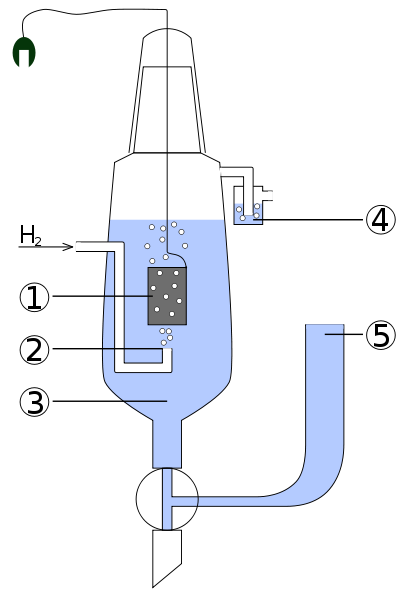
\includegraphics[keepaspectratio,width=3cm]{img/SVE.png}
		\end{figure}
	\end{columns}
}

\section{Magnetické vlastnosti látek}
\frame{
	\frametitle{}
	\vfill
	\begin{columns}
		\begin{column}{.75\textwidth}
			\begin{itemize}
				\item Podle chování v magnetickém poli rozlišujeme látky:\footnote[frame]{\href{http://fyzika.jreichl.com/main.article/view/295-magneticke-vlastnosti-latek}{Magnetické vlastnosti látek}}
				\begin{itemize}
					\item diamagnetické
					\item paramagnetické
					\item feromagnetické
					\item ferimagnetické
					\item antiferomagnetické
					\item altermagnetické
				\end{itemize}
				\item \textit{Diamagnetické látky} vypuzují magnetické pole ze svého objemu.
				\item Jsou složeny z atomů, které neobsahují nepárové elektrony.
				\begin{itemize}
					\item Ideálními diamagnetiky jsou supravodiče I. typu.
				\end{itemize}
				\item Diamagnetické jsou zlato, měď nebo rtuť. Za laboratorní teploty je  jedním z nejsilnějších diamagnetických materiálů pyrolytický uhlík.\footnote[frame]{\href{https://www.kjmagnetics.com/blog.asp?p=diamagnetic-levitation}{Diamagnetism and Levitation}}
			\end{itemize}
		\end{column}
		\begin{column}{.4\textwidth}
			\begin{figure}
				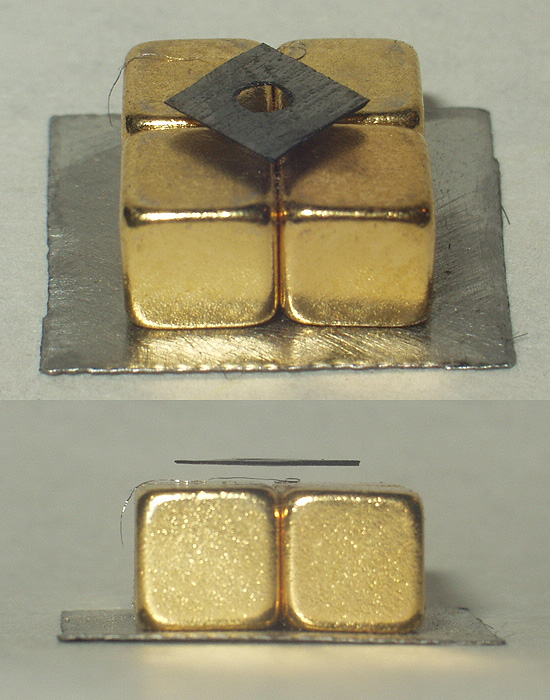
\includegraphics[width=.95\textwidth]{img/Diamagnetic_graphite_levitation.jpg}
				\caption*{Pyrolytický grafit levitující nad magnetem.\footnote[frame]{\href{https://commons.wikimedia.org/wiki/File:Diamagnetic_graphite_levitation.jpg}{Zdroj: Splarka/Commons}}}
			\end{figure}
		\end{column}
	\end{columns}
	\vfill
}

\frame{
	\frametitle{}
	\vfill
	\begin{columns}
		\begin{column}{.7\textwidth}
			\begin{itemize}
				\item \textit{Paramagnetické látky} mají ve své struktuře nepárové elektrony.
				\item Jsou přitahovány vnějším magnetickým polem.
				\item Příkladem je hliník, vápník nebo hořčík.
				\item \textit{Feromagnetické látky} jsou složeny z paramagnetických atomů uspořádaných do magnetických domén.
				\item Ty jsou orientovány náhodně, ale v přítomnosti magnetického pole se všechny orientují shodně s vnějším polem.
				\item Dokáží si udržet magnetismus i v nepřítomnosti magnetického pole.
				\item Feromagnetické látky se využívají při konstrukci jader cívek v elektromagnetech a transformátorech.\footnote[frame]{\href{https://kke.zcu.cz/export/sites/kke/about/projekty/enazp/projekty/09_Silnoprouda-zarizeni_24-26/24_IUT/052_Transformatory---Picmausova---P1.pdf}{Transformátory}}
			\end{itemize}
		\end{column}
		\begin{column}{.4\textwidth}
			\begin{figure}
				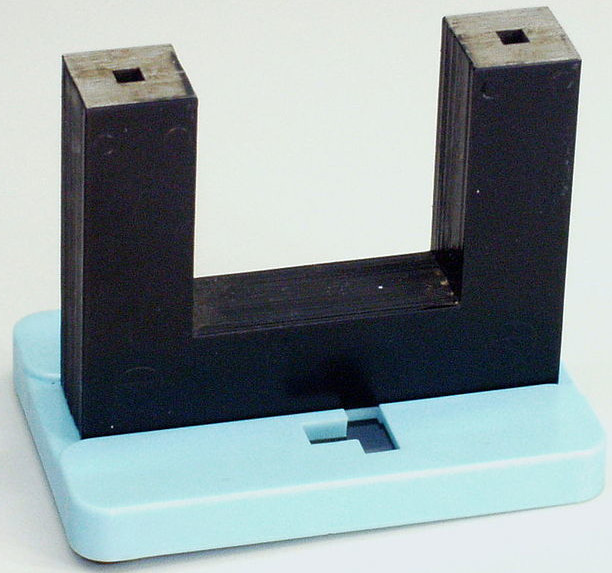
\includegraphics[width=\textwidth]{img/Trafo.jpg}
				\caption*{Jádro transformátoru.\footnote[frame]{\href{https://commons.wikimedia.org/wiki/File:Trafo_1.jpg}{Zdroj: Zátonyi Sándor/Commons}}}
			\end{figure}
		\end{column}
	\end{columns}
	\vfill
}

\frame{
	\frametitle{}
	\vfill
	\begin{itemize}
		\item Při zahřátí nad tzv. \textit{Curieovu teplotu} dojde k rozpadu domén a materiál přestane být feromagnetikem.
	\end{itemize}
	\begin{center}
		\begin{tabular}{|l|r@{}l|}
			\hline
			\textbf{Materiál} &
			\multicolumn{2}{|l|}{\textbf{Curieova teplota [$^\circ$C]}} \\\hline
			Kobalt & & 1115 \\\hline
			Železo & & 770 \\\hline
			Oxid železitý & & 675 \\\hline
			Nikl & & 354 \\\hline
			Gadolinium & & 19 \\\hline
			Terbium & $-$ & 54 \\\hline
			Dysprosium & $-$ & 185 \\\hline
		\end{tabular}
	\end{center}
	\vfill
}

\frame{
	\frametitle{}
	\vfill
	\begin{itemize}
		\item \textit{Ferimagnetické látky} mají menší část spinů orientovanou opačným směrem než působí magnetické pole.
		\item Mají také vyšší elektrický odpor než feromagnetické látky.
		\item Jde např. o \ce{Fe2O3} nebo \ce{MnO}.
		\item \textit{Antiferomagnetické látky} mají také magnetické domény, ale ty jsou orientovány opačně a navzájem se nulují.\footnote[frame]{\href{https://www.tcd.ie/Physics/research/groups/magnetism/files/lectures/5006/5006-6.pdf}{Antiferromagnetism and Other Magnetic Ordeer)}}
		\item Po překročení tzv. \textit{Néelovy teploty} se mění na paramagnetické látky.\footnote[frame]{\href{https://www.differencebetween.com/difference-between-curie-temperature-and-neel-temperature/}{Difference Between Curie Temperature and Neel Temperature}}
		\item Většina látek vykazuje antiferomagnetismus za nízkých teplot.
		\item Jediným antiferomagnetickým prvkem za laboratorní teploty je chrom.\footnote[frame]{\href{https://doi.org/10.1103/RevModPhys.60.209}{Spin-density-wave antiferromagnetism in chromium)}}
	\end{itemize}
	\vfill
}

\frame{
	\frametitle{}
	\vfill
	\begin{itemize}
		\item \textit{Altermagnetické látky} jsou kombinací ferromagnetických a antiferomagnetických látek.
		\item Střídají se nejen směry magnetických momentů na sousedních atomech, ale také se střídá prostorová orientace atomů v krystalu.\footnote[frame]{\href{https://physics.aps.org/articles/v17/4}{Altermagnetism Then and Now}}
		\item Altermagnetismus byl teoreticky popsán v roce 2019 a prakticky prokázán v roce 2023 vědci z AV ČR.\footnote[frame]{\href{https://www.avcr.cz/cs/pro-media/tiskove-zpravy/Vedci-experimentalne-potvrdili-altermagnetismus/}{Vědci experimentálně potvrdili altermagnetismus}}
	\end{itemize}
	\vfill
}

\section{Periodická soustava prvků}
\frame{
	\frametitle{}
	\begin{center}
		\adjincludegraphics[width=1.1\textwidth]{../IUPAC_PSP.jpg}
	\end{center}
}

\frame{
	\frametitle{}
	\vfill
	\begin{itemize}
		\item Prvky jsou uspořádány podle vzrůstajícího atomového čísla.
		\item Jsou uspořádány do skupin a period.
		\item Ve \emph{skupinách} jsou prvky se stejným počtem valenčních elektronů. Díky podobné elektronové konfiguraci mají podobné chemické vlastnosti. Skupin je celkem 18.
		\item V \emph{periodách} jsou prvky jejichž valenční elektrony obsazují stejnou energetickou hladinu. Všechny dosud známé prvky jsou v periodách 1---8.
		\item Dále můžeme prvky rozdělit do čtyřech \emph{bloků}, podle typu orbitalu, který obsadil poslední elektron. Známe čtyři bloky - s, p, d a f.
		\item  Podle fyzikálních a chemických vlastností rozdělujeme prvky do tří velkých skupin --- kovy, polokovy a nekovy.
	\end{itemize}
	\vfill
}

\subsection{Skupiny}
\frame{
	\frametitle{}
	\vfill
	\begin{itemize}
		\item 1. skupina (Alkalické kovy): \textbf{H}ana \textbf{Lí}bá \textbf{Na} \textbf{K}řižovatce \textbf{R}o\textbf{b}ustního \textbf{C}e\textbf{s}táře \textbf{Fr}antu
		\item 2. skupina (Kovy alkalických zemin): \textbf{Bě}žela \textbf{M}a\textbf{g}da \textbf{Ca}ňonem, \textbf{Sr}azila \textbf{Ba}nán \textbf{Ra}menem
		\item 13. skupina (Triely): \textbf{B}yl \textbf{Al}exej \textbf{Ga}garin \textbf{In}dickým \textbf{Tl}umočníkem?
		\item 14. skupina (Tetrely): \textbf{C}opak \textbf{Si} \textbf{Ge}rtruda \textbf{Sn}ědla \textbf{P}lom\textbf{b}u
		\item 15. skupina (Pentely): \textbf{N}áš \textbf{P}an \textbf{As}istent \textbf{Sb}írá \textbf{Bi}kiny
		\item 16. skupina (Chalkogeny): \textbf{Ó} \textbf{S}lečny \textbf{Se}jměte \textbf{Te}nké \textbf{Po}dkolenky
		\item 17. skupina (Halogeny): \textbf{F}ranta \textbf{Cl}oumal \textbf{Br}omem \textbf{J}ako \textbf{At}let
		\item 18. skupina (Inertní plyny): \textbf{He}lena \textbf{Ne}se \textbf{Ar}ašídy \textbf{Kr}áli \textbf{Xe}nonu \textbf{Rá}no
	\end{itemize}
	\vfill
}

\section{Elektronová konfigurace}
\frame{
	\frametitle{}
	\begin{itemize}
		\item Popisuje zaplnění atomových orbitalů elektrony
		\item Orbitaly jsou zaplňovány v pořadí: 1s, 2s, 2p, 3s, 3p, 4s, 3d, 4p, 5s, 4d, 5p, 6s, 4f, 5d, 6p, 7s, 5f, 6d, 7p
		\item d-orbitaly se zaplňují až po zaplnění s-orbitalu s hlavním kvantovým číslem (n+1), např. 3d orbital se začne plnit až po 4s
		\item Zápis elektronové konfigurace: C: 1s$^2$ 2s$^2$ 2p$^2$; P: 1s$^2$ 2s$^2$ 2p$^6$ 3s$^2$ 3p$^3$
		\item Zkrácený zápis elektronové konfigurace: C: [He] 2s$^2$ 2p$^2$; P: [Ne] 3s$^2$ 3p$^3$
		\item U nepřechodných prvků (s a p blok PSP) je zaplňování orbitalů dáno jejich energetickým pořadím. Sb: [Kr] 4d$^{10}$ 5s$^2$ 5p$^3$
		\item U přechodných (d blok) a vnitřně přechodných (f blok) prvků nacházíme výjimky a nepravidelnosti v pořadí zaplňování orbitalů
	\end{itemize}
}

\frame{
	\frametitle{}
	\begin{itemize}
		\item \textbf{Změna pořadí energetických hladin}
	\end{itemize}

	\begin{tabular}{l|l}
		K & [Ar] 4s$^1$ (3d$^0$ 4p$^0$) \\
		Ca & [Ar] 4s$^2$ (3d$^0$ 4p$^0$) \\
		\hline \hline
		Sc & [Ar] 3d$^1$ 4s$^2$ (4p$^0$) \\
		Ti & [Ar] 3d$^2$ 4s$^2$ (4p$^0$) \\
	\end{tabular}

	\begin{itemize}
		\item \textbf{Vyšší stabilita zpola zaplněných d-orbitalů}
		\item U prvků 6. a 11. skupiny dochází k přeskoku jednoho elektronu z~orbitalu s do orbitalu d, tím vzniká konfigurace se zpola nebo zcela zaplněným d-orbitalem.
		\item Cr: [Ar]  3d$^5$ 4s$^1$
		\item Cu: [Ar]  3d$^{10}$ 4s$^1$
	\end{itemize}
}

\frame{
	\frametitle{}
	\begin{itemize}
		\item U f-prvků, \textbf{lanthanoidů}, je elektronová konfigurace  4f$^{1-14}$ 5d$^0$ 6s$^2$
		\item Výjimkou je cer, který má konfiguraci 4f$^1$ 5d$^1$ 6s$^2$. To je dáno malým rozdílem energií mezi 4f a 5d orbitalem.
		\item Druhou výjimkou je gadolinium s konfigurací 4f$^7$ 5d$^1$ 6s$^2$, to je způsobeno vyšší stabilitou konfigurace 4f$^7$.
		\item Elektronová konfigurace \textbf{aktinoidů} se řídí složitějšími pravidly.
		\item Orbitaly 5f se začínají zaplňovat až od protaktinia.
		\item Ac: 6d$^1$ 7s$^2$
		\item Th: 6d$^2$ 7s$^2$
		\item Pa: 5f$^2$ 6d$^1$ 7s$^2$ nebo 5f$^1$ 6d$^2$ 7s$^2$
		\item Cf: 5f$^{10}$ 7s$^2$
	\end{itemize}
	\begin{figure}
		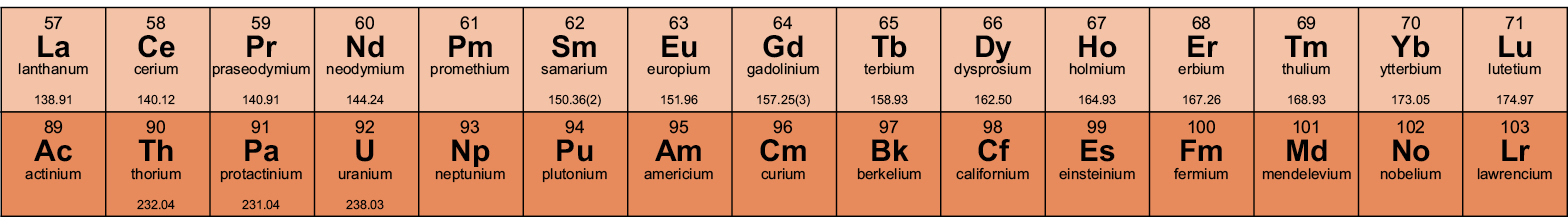
\includegraphics[width=\textwidth]{img/F-block.jpg}
	\end{figure}
}

%http://www.imaturita.cz/maturitni-otazky/chemie/periodicka-tabulka/397/
\section{Periodicita vlastností prvků}
\frame{
	\frametitle{}
	\vfill
	\begin{itemize}
		\item Vlastnosti prvků odpovídají umístění prvku v PSP. Podobnost prvků v rámci skupiny PSP je dána podobnou konfigurací valenční elektronové vrstvy.\footnote[frame]{\href{http://chemwiki.ucdavis.edu/Inorganic_Chemistry/Descriptive_Chemistry/Periodic_Trends_of_Elemental_Properties/Periodic_Trends}{Periodic Trends} na UCDavis Chemwiki}
		\item \textbf{Atomový poloměr} v periodě klesá s rostoucím protonovým číslem, je to dáno zvyšujícím se nábojem jádra, které pak silněji přitahuje elektrony zaplňující valenční slupku. V rámci skupiny roste se stoupajícím protonovým číslem.
		\item \textbf{Elektronegativita} v periodě narůstá, ve skupině postupně klesá.
		\item \textbf{Ionizační energie} klesá v rámci skupiny, v rámci periody roste.
		\item \textbf{Redoxní vlastnosti} v levé části tabulky jsou redukční činidla (H, Na, Ca, Mg) a v pravé oxidační (F, O, Cl).
		\item \textbf{Acidobazické vlastnosti} v levé části tabulky jsou zásadotvorné prvky (Na, K, Ca, Mg) a v pravé kyselinotvorné (F, Cl, S).
	\end{itemize}
	\vfill
}

\frame{
	\frametitle{}
	\vfill
	\begin{figure}
		\begin{figure}
			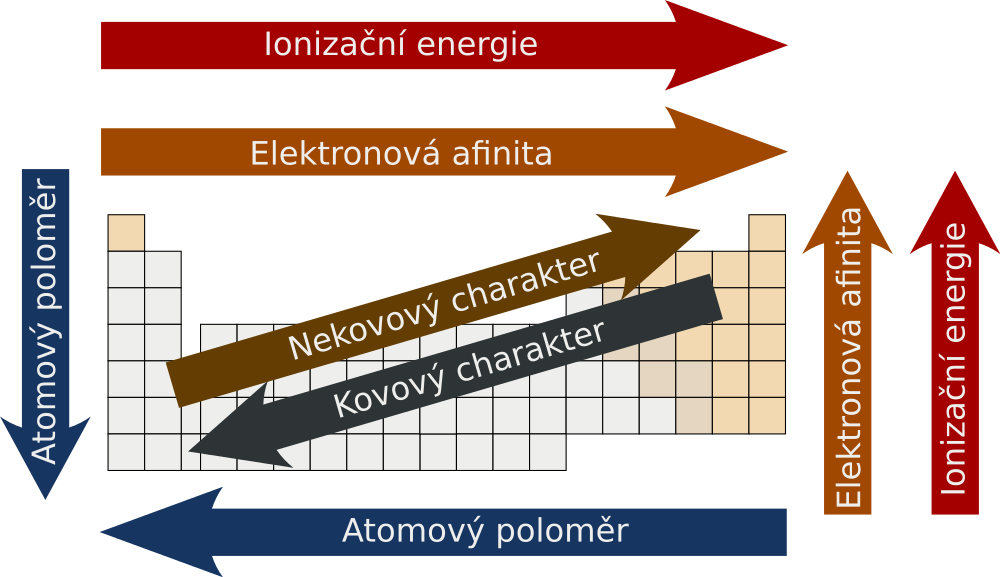
\includegraphics[height=.65\textheight]{img/Periodicky_zakon.png}
			\caption*{Periodicita vlastností prvků.\footnote[frame]{\href{https://commons.wikimedia.org/wiki/File:Periodicky_zakon.svg}{Zdroj: Mirek2/Commons}}}
		\end{figure}
	\end{figure}
	\vfill
}

\subsection{Atomové poloměry}
\frame{
	\frametitle{}
	\vfill
	\begin{figure}
		\begin{figure}
			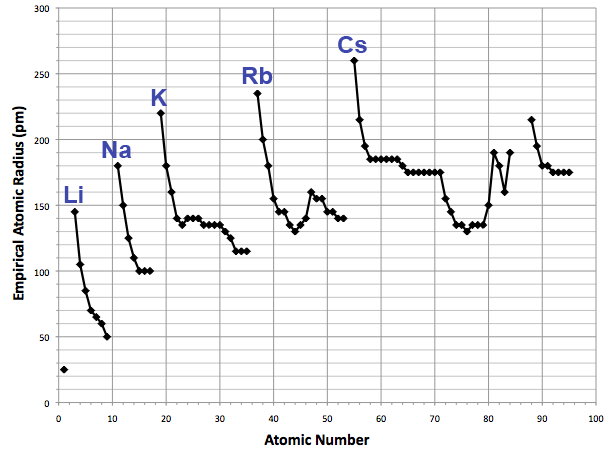
\includegraphics[height=.65\textheight]{img/Empirical_atomic_radius_trends.png}
			\caption*{Závislost atomového poloměru na protonovém čísle.\footnote[frame]{\href{https://commons.wikimedia.org/wiki/File:Empirical_atomic_radius_trends.png}{Zdroj: StringTheory11/Commons}}}
		\end{figure}
	\end{figure}
	\vfill
}

\subsection{Atomové a iontové poloměry}
\frame{
	\frametitle{}
	\vfill
	\begin{figure}
		\begin{center}
			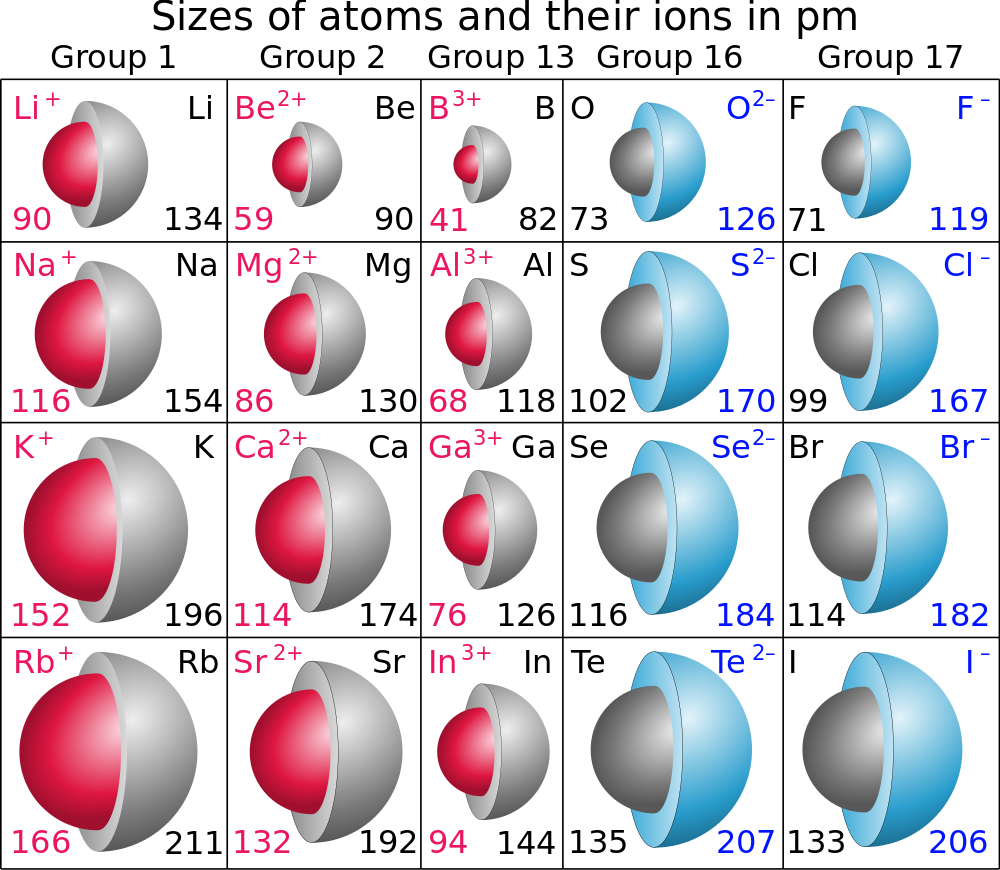
\includegraphics[height=.65\textheight]{img/Atomic_and_ionic_radii.png}
			\caption*{Atomové a iontové poloměry.\footnote[frame]{\href{https://commons.wikimedia.org/wiki/File:Atomic_\%26_ionic_radii.svg}{Zdroj: Popnose/Commons}}}
		\end{center}
	\end{figure}
	\vfill
}

\subsection{Lanthanoidová a aktinoidová kontrakce}
\frame{
	\frametitle{}
	\vfill
	\begin{itemize}
		\item \textit{Lanthanoidová kontrakce} je jev, kdy dochází se stoupajícím protonovým číslem lanthanoidů ke zmenšování iontového poloměru.
		\item Tento jev je způsoben slabším stíněním elektronů v orbitalech \textit{4f}.
		\item S přibývajícím počtem protonů v jádře tak roste přitažlivá síla působící na jednotlivé elektrony.
		\item Iontový poloměr \ce{La^{3+}} je 103~pm, zatímco pro \ce{Lu^{3+}} je to jen 86~pm.
	\end{itemize}

	\begin{tabular}{|*{9}{l|}}
		\hline
		Prvek & La & Ce & Pr & Pm & Eu & Tb & Ho & Lu \\\hline
		Ion. polom. \ce{M^{3+}} [pm] & 103 & 102 & 99 & 97 & 94,7 & 92,3 & 90,1 & 86,1 \\\hline
	\end{tabular}

	\begin{itemize}
		\item Tento vliv lze pozorovat i v jiných skupinách prvků, např. iontový poloměr \ce{Zr^{4+}} je 79~pm a pro \ce{Hf^{4+}} je 78~pm.
		\item Podobný jev pozorujeme i u aktinoidů, kde se označuje jako \textit{aktinoidová kontrakce}.
	\end{itemize}

	\begin{tabular}{|*{9}{l|}}
		\hline
		Prvek & Pa & U & Np & Pu & Am & Cm & Bk & Cf \\\hline
		Ion. polom. \ce{M^{3+}} [pm] & 104 & 102,5 & 101 & 100 & 97,5 & 97 & 96 & 95 \\\hline
		Ion. polom. \ce{M^{4+}} [pm] & 90 & 89 & 87 & 86 & 85 & 85 & 83 & 82,1 \\\hline
	\end{tabular}
	\vfill
}

\subsection{První ionizační energie}
\frame{
	\frametitle{}
	\vfill
	\begin{itemize}
		\item \textit{Ionizační energie} atomu je energie, kterou musíme vynaložit na odtržení elektronu.
		\item Hodnota první ionizační energie ve skupinách klesá s rostoucím protonovým číslem, v periodách pak roste.
		\item Ionizační energie je dána z velké části energií orbitalu, ve kterém je elektron umístěn.
	\end{itemize}
	\begin{figure}
		\begin{figure}
			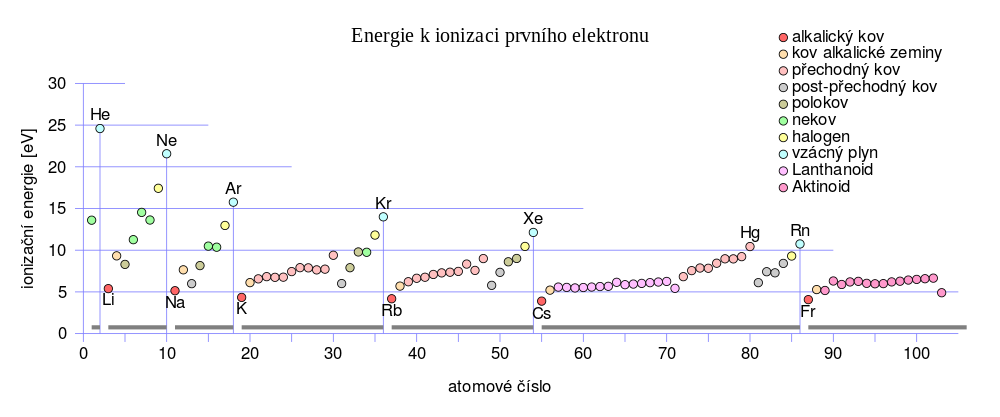
\includegraphics[width=.9\textwidth]{img/First_Ionization_Energy.png}
			\caption*{První ionizační energie.\footnote[frame]{\href{https://commons.wikimedia.org/wiki/File:First_Ionization_Energy.svg}{Zdroj: Sponk/Commons}}}
		\end{figure}
	\end{figure}
	\vfill
}

\subsection{Elektronová afinita}
\frame{
	\frametitle{}
	\vfill
	\begin{itemize}
		\item \textit{Elektronová afinita} je energie, která se uvolní při vzniku aniontu.
		\item \ce{A (g) + e^- -> A^- (g)}
		\item Čím je anion stabilnější, tím je i vyšší hodnota elektronové afinity.
		\item Elektronová afinita roste v rámci periody, což je způsobeno postupným zaplňováním elektronové slupky.
	\end{itemize}
	\begin{figure}
		\begin{figure}
			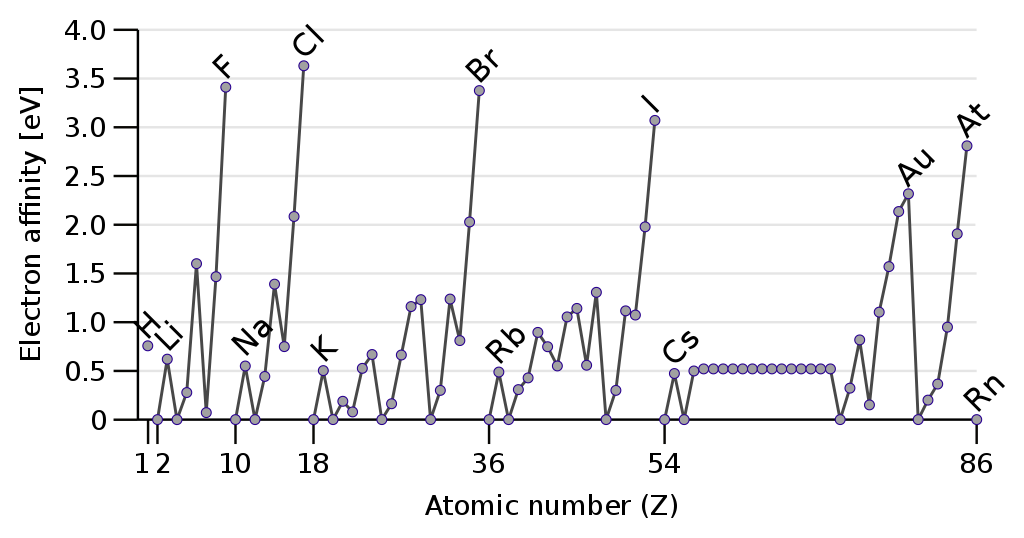
\includegraphics[width=.75\textwidth]{img/Electron_affinity_of_the_elements.png}
			\caption*{Elektronové afinity.\footnote[frame]{\href{https://commons.wikimedia.org/wiki/File:Electron_affinity_of_the_elements.svg}{Zdroj: DePiep/Commons}}}
		\end{figure}
	\end{figure}
	\vfill
}

\subsection{Inertní elektronový pár}
\frame{
	\frametitle{}
	\vfill
	\begin{itemize}
		\item Efekt inertního páru je jev, kdy se elektrony v orbitalu \textit{s} valenční slupky nezapojují do tvorby chemických vazeb.\footnote[frame]{\href{http://www.chemguide.co.uk/inorganic/group4/oxstates.html}{Oxidation state trends in group 4}}
		\item Projevuje se to vyšší stabilitou nižšího oxidačního stavu oproti lehčím prvků.
		\item Efekt pozorujeme u těžších prvků skupin 13--16.
		\item Prvky p bloku ve 4.-6. periodě mají díky vlivu d- a f- orbitalů pevněji vázané s-elektrony valenční slupky.
		\item Efekt můžeme ilustrovat nízkou stabilitou sloučenin \ce{Pb^{IV}} oproti \ce{Sn^{IV}}.
		\item Efekt se může projevovat i nízkou sterickou aktivitou tohoto elektronového páru, tzn. že pár neovlivňuje geometrii sloučeniny (nelze pak použít teorii VSEPR).
	\end{itemize}
	\vfill
}

\subsection{Allotropie prvků}
\frame{
	\frametitle{}
	\vfill
	\begin{itemize}
		\item Koncept \textit{alotropie} navrhl v roce 1841 Jöns Jakob Berzelius, termín je odvozen z řeckého pro variabilitu.\footnote[frame]{\href{https://doi.org/10.1021/ed083p838}{The Origin of the Term Allotrope}}
		\item Alotropy prvku jsou rozdílné strukturní modifikace daného prvku, mají odlišné fyzikální i chemické vlastnosti.\footnote[frame]{\href{http://www.chemistryexplained.com/A-Ar/Allotropes.html}{Allotropes}}
		\item S alotropy se setkáváme např. u uhlíku, fosforu, síry a mnoha dalších prvků.
		\begin{itemize}
			\item \textit{Uhlík}: diamant, grafit, grafen, fullereny, uhlíkové nanotrubice, $\ldots$
			\item \textit{Fosfor}: bílý, červený, černý, fialový
			\item \textit{Selen}: červený, šedý, černý
			\item \textit{Kobalt}: $\alpha$-kobalt, $\beta$-kobalt
		\end{itemize}
	\end{itemize}
	\begin{figure}
		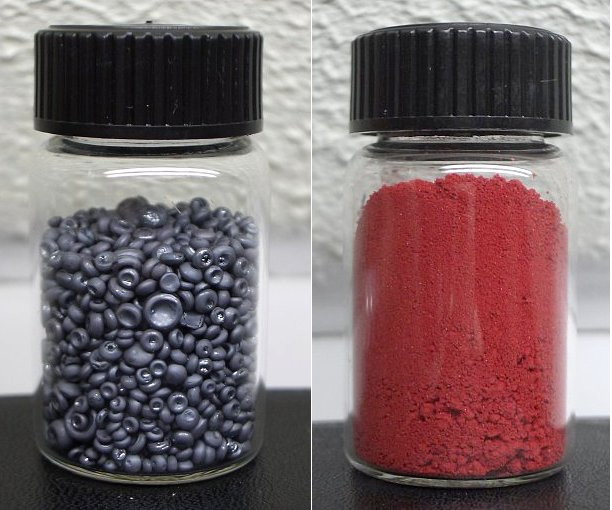
\includegraphics[height=.2\textheight]{img/SeBlackRed.jpg}
		\caption*{Černý a červený selen.\footnote[frame]{Zdroj: \href{https://commons.wikimedia.org/wiki/File:SeBlackRed.jpg}{W. Oelen/Commons}}}
	\end{figure}
	\vfill
}

\subsection{Polymorfie}
\frame{
	\frametitle{}
	\vfill
	\begin{columns}
		\begin{column}{.6\textwidth}
			\begin{itemize}
				\item \textit{Polymorfie} (mnohotvarost) je ekvivalent alotropie u sloučenin. Je to schopnost látek krystalovat ve více krystalových strukturách.
				\item \textit{Polymorfní přechod} je reverzibilní přechod mezi polymorfními modifikacemi. Nedochází tedy ke změně chemického složení, ale pouze uspořádání v krystalu.
				\item Polymorfii pozorujeme u organických (benzamid, kyselina maleinová) i anorganických sloučenin (křemen, oxid hlinitý, oxid chromitý).
			\end{itemize}
		\end{column}
		\begin{column}{.45\textwidth}
			\begin{figure}
				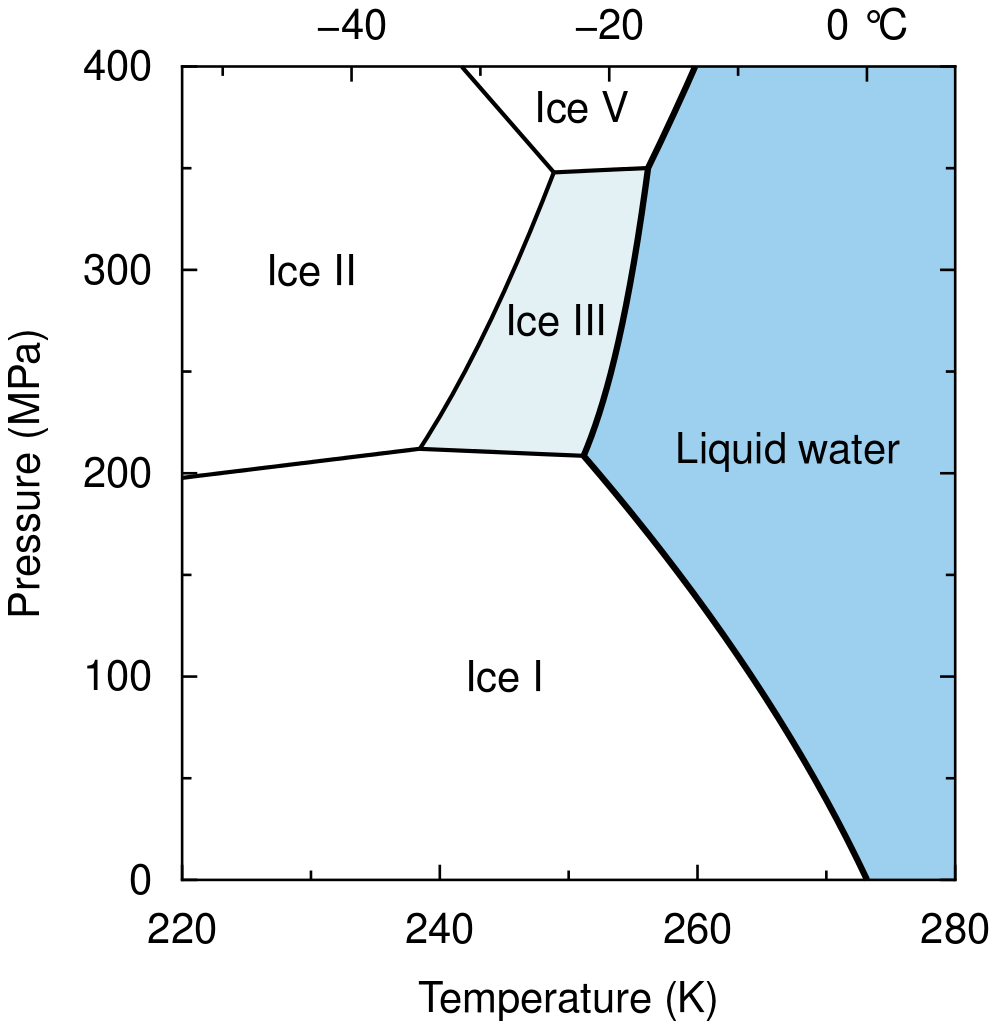
\includegraphics[width=\textwidth]{img/Ice_III_phase_diagram.png}
				\caption*{Fázový diagram vody.\footnote[frame]{Zdroj: \href{https://commons.wikimedia.org/wiki/File:Ice_III_phase_diagram.svg}{Cavit/Commons}}}
			\end{figure}
		\end{column}
	\end{columns}
	\vfill
}

\frame{
	\frametitle{}
	\vfill
	\begin{columns}
		\begin{column}{.5\textwidth}
			\begin{figure}
				\includegraphics[width=\textwidth]{img/Α-Quartz.png}
				\caption*{$\alpha$-křemen (trigonální).\footnote[frame]{Zdroj: \href{https://commons.wikimedia.org/wiki/File:A-quartz.png}{Materialscientist/Commons}}}
			\end{figure}
		\end{column}
		\begin{column}{.5\textwidth}
			\begin{figure}
				\includegraphics[width=\textwidth]{img/Β-Quartz.png}
				\caption*{$\beta$-křemen (hexagonální).\footnote[frame]{Zdroj: \href{https://commons.wikimedia.org/wiki/File:B-quartz.png}{Materialscientist/Commons}}}
			\end{figure}
		\end{column}
	\end{columns}
	\vfill
}

\section{VSEPR}
\frame{
	\frametitle{}
	\begin{itemize}
		\item \textbf{V}alence \textbf{S}hell \textbf{E}lectron \textbf{P}air \textbf{R}epulsion
		\item Tvar molekuly určíme na základě rozmístění elektronových párů v okolí centrálního atomu tak, aby jejich vzájemné odpuzování bylo co nejmenší.
		\item Tento model je vhodný převážně pro sloučeniny nepřechodných prvků.
		\item Uvažujeme pouze nevazebné elektronové páry - $n$ a vazebné elektronové páry $\sigma$.
		\item \textbf{Základní pravidla VSEPRu}
		\begin{enumerate}
			\item Elektronové páry centrálního atomu se v prostoru rozmístí tak, aby byly co nejdále od sebe a měly minimální energii.
			\item Nevazebný elektronový pár odpuzuje ostatní elektronové páry nejvíce, odpuzování  vazebných elektronových párů je slabší a klesá v pořadí trojná vazba $>$ dvojná vazba $>$ jednoduchá vazba.
			\item Tvar molekuly je dán pouze polohou vazebných elektronových párů.
		\end{enumerate}
		\item Pro určení tvaru klastrů se využívá teorie PSEPT (Polyhedral Skeletal Electron Pair Theory).\footnote[frame]{\href{https://dx.doi.org/10.1007/BFb0018033}{Clusters with interstitial atoms from the p-block: How do Wade's rules handle them?}}
	\end{itemize}
}

\frame{
	\frametitle{}
	\begin{itemize}
		\item Postup pro určení tvaru molekuly pomocí teorie VSEPR:
		\begin{enumerate}
			\item Vytvoříme elektronový strukturní vzorec molekuly nebo iontu.
			\item Určíme počet $\sigma$ vazeb vycházejících z centrálního atomu (n$_\sigma$).
			\item Určíme počet nevazebných elektronových párů na centrálním atomu (n$_{nev}$).
			\item Určíme obecný vzorec molekuly ve tvaru \ce{AX_\sigma E_{nev}}.
			\item Podle obecného vzorce zvolíme tvar a poté určíme deformace molekuly od ideálního tvaru.
		\end{enumerate}
		\item Deformace molekuly jsou dány:
		\begin{enumerate}
			\item rozdílným řádem vazby.
			\item rozdílnou elektronegativitou atomů tvořících vazby, čímž dochází k nerovnoměrnému rozmístění elektronové hustoty ve vazbě.
		\end{enumerate}
	\end{itemize}
}

\subsection{Výchozí tvary}
\frame{
	\frametitle{}
	\begin{tabular}{|c|c|c|}
		\hline
		Počet elektronových párů & \multicolumn{2}{|c|}{Tvar} \\\hline
		2 & lineární &\color{red} X---A---X \\\hline
		3 & trojúhelník &  \raisebox{-.9\height}{\adjincludegraphics[width=20mm]{img/AX3.png}} \\[40pt]
		\hline
		4 & tetraedr & \raisebox{-.9\height}{\adjincludegraphics[width=20mm]{img/AX4.png}} \\[40pt]
		\hline
	\end{tabular}
}

\frame{
	\frametitle{}
	\begin{tabular}{|c|c|c|}
		\hline
		Počet elektronových párů & \multicolumn{2}{|c|}{Tvar} \\\hline
		5 & trigonální bipyramida & \raisebox{-.9\height}{\adjincludegraphics[width=20mm]{img/AX5.png}} \\[65pt]
		\hline
		6 & oktaedr & \raisebox{-.9\height}{\adjincludegraphics[width=20mm]{img/AX6.png}} \\[65pt]
		\hline
	\end{tabular}
}

\subsection{Dva elektronové páry na centrálním atomu}
\frame{
	\frametitle{}
	Pokud centrální atom (A) nese dva elektronové páry, je tvar molekuly vždy lineární. Pokud jsou oba vazebné (X), označujeme molekulu jako \ce{AX2}, pokud je jeden nevazebný (E), označení je \ce{AXE}.
	\\
	\hrule
	\vspace{5mm}
	\ce{AX2}
	\\
	\vspace{5mm}
	{\LARGE\color{red} X---A---X}
	\vspace{5mm}

	Tvar: lineární; $\angle XAX = 180^\circ$; Příklad: \ce{CO2}, \ce{BeF2}
	\vspace{5mm}
	\hrule
	\vspace{5mm}
	\ce{AXE}

	\vspace{5mm}
	{\LARGE E---\color{red} A---X}
	\vspace{5mm}


	Tvar: lineární; $\angle EAX = 180^\circ$;  Příklad: CO
}

\subsection{Tři elektronové páry na centrálním atomu}
\frame{
	\frametitle{}

	\ce{AX3}

	\adjincludegraphics[width=30mm]{img/AX3.png}

	Tvar:  rovnostranný trojúhelník; $\angle XAX = 120^\circ$
	Příklad: \ce{BCl3}
}

\frame{
	\frametitle{}

	\ce{AX2E}
	\begin{columns}
		\column{.35\textwidth}
		\adjincludegraphics[width=30mm]{img/AX2E.png}
		\column{.65\textwidth}
		Tvar: lomený; $\angle XAX < 120^\circ$
		Příklad: \ce{SO2}
	\end{columns}
	\vspace{5mm}
	\hrule
	\vspace{2mm}
	\ce{AXE2}
	\begin{columns}
		\column{.35\textwidth}
		\adjincludegraphics[width=30mm]{img/AXE2.png}
		\column{.65\textwidth}
		Tvar: lineární; Příklad: \ce{O2}
	\end{columns}
}

\subsection{Čtyři elektronové páry na centrálním atomu}
\frame{
	\frametitle{}
	\begin{tabular}{|c|c|c|}
		\ce{AX4} & \ce{AX3E} & \ce{AX2E2} \\
		\adjincludegraphics[width=25mm]{img/AX4.png} &
		\adjincludegraphics[width=25mm]{img/AX3E.png} &
		\adjincludegraphics[width=25mm]{img/AX2E2.png} \\
		Tvar: tetraedr & trigonální pyramida & lomený \\
		$\angle XAX = 109.5^\circ$ & $\angle XAX < 109.5^\circ$ & $\angle XAX << 109.5^\circ$ \\
		Příklad: \ce{SO^{2-}_4} & \ce{PH3} &  \ce{SeBr2} \\
	\end{tabular}
}

\subsection{Pět elektronových párů na centrálním atomu}
\frame{
	\frametitle{}
	\scalebox{0.93}{
		\begin{tabular}{|c|c|c|c|}
			\ce{AX5} & \ce{AX4E} & \ce{AX3E2} & \ce{AX2E3} \\
			\adjincludegraphics[width=20mm]{img/AX5.png} &
			\adjincludegraphics[width=20mm]{img/AX4E.png} &
			\adjincludegraphics[width=20mm]{img/AX3E2.png} &
			\adjincludegraphics[width=20mm]{img/AX2E3.png} \\

			Tvar: trigonální  & houpačka & tvar T & lineární \\
			bipyramida &&&\\
			$\angle XAX = 90^\circ \ a\ 120^\circ$ & $\angle XAX < 90^\circ$ a $< 120^\circ$ & $\angle XAX = 90^\circ$
			& $\angle XAX = 180 ^\circ$ \\
			Příklad: \ce{AsF5} & \ce{SeH4} &  \ce{ICl3} &  \ce{BrF2^-} \\
		\end{tabular}
	}%end scalebox
}

\subsection{Šest elektronových párů na centrálním atomu}
\frame{
	\frametitle{}
	\begin{tabular}{|c|c|c|}
		\ce{AX6} & \ce{AX5E} & \ce{AX4E2} \\
		\adjincludegraphics[width=25mm]{img/AX6.png} &
		\adjincludegraphics[width=25mm]{img/AX5E.png} &
		\adjincludegraphics[width=25mm]{img/AX4E2.png} \\
		Tvar: oktaedr & čtvercová pyramida & čtverec \\
		$\angle XAX = 90^\circ$ & $\angle XAX < 90^\circ$ & $\angle XAX = 90^\circ$ \\
		Příklad: \ce{SF6} & \ce{IF5} &  \ce{XeF4} \\
	\end{tabular}
}

\section{Symetrie molekul}
\frame{
	\frametitle{}
	\vfill
	\begin{itemize}
		\item \textbf{Operace symetrie} - geometrická operace, jejímž provedením dostaneme objekt do polohy nerozlišitelné od výchozí.
		\item \textbf{Prvek symetrie} - body, jejichž poloha se v průběhu provádění operace symetrie nemění.
		\item U molekul existuje pět prvků symetrie.
	\end{itemize}

	\begin{tabular}{|l|l|l|}
		\hline
		\textbf{Operace symetrie} & \textbf{Symbol} & \textbf{Prvek symetrie} \\
		\hline
		Identita & E & Celý objekt \\
		\hline
		Rotace & $C_n$ & Rotační osa \\
		\hline
		Zrcadlení & $\sigma$ & Rovina symetrie \\
		\hline
		Inverze & i & Střed symetrie \\
		\hline
		Nevlastní osa & $S_n$ & Rotačně-reflexní osa \\
		\hline
	\end{tabular}
	\vfill
}

\section{Dipólový moment}
\frame{
	\frametitle{}
	\vfill
	\begin{itemize}
		\item Vektor popisující rozložení elektrického náboje v molekule.
		\item Výsledný dipólmoment získáme vektorovým součtem dipólmomentů jednotlivých vazeb.
		\item Pro dvojatomové molekuly je definován jako součin parciálního náboje na kladně nabitém atomu a mezijaderné vzdálenosti:
		\item $\vec{\mu} = \vec{\delta} . l$ [C.m]
	\end{itemize}
	\begin{columns}
		\begin{column}{0.6\textwidth}
			\begin{figure}
				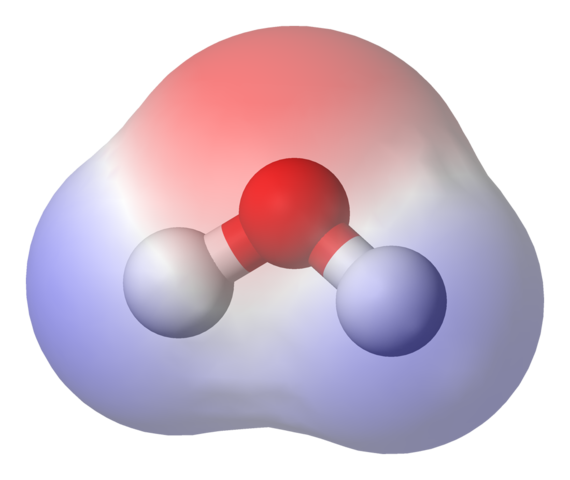
\includegraphics[height=.4\textheight]{img/water-elpot.png}
				\caption*{Rozložení elektronové hustoty v molekule vody.\footnote[frame]{\href{https://commons.wikimedia.org/wiki/File:Water-elpot-transparent-3D-balls.png}{Zdroj: Benjah-bmm27/Commons}}}
			\end{figure}
		\end{column}

		\begin{column}{0.4\textwidth}
			\begin{figure}
				\begin{picture}(0,0)(20,-50)
					\color{red}
					\put(0,0){O}
					\color{blue}
					\put(23,-30){H}
					\put(-23,-30){H}
					\color{black}
					\thicklines
					\put(24,-21){\vector(-1,1){20}}
					\put(-16,-21){\vector(1,1){20}}
					\color{green}
					\put(4,-41){\vector(0,1){40}}
					\color{black}
					\thinlines
					\put(24,-21){\line(-1,-1){20}}
					\put(-16,-21){\line(1,-1){20}}
				\end{picture}
			\end{figure}
		\end{column}
	\end{columns}
	\vfill
}

\section{Koordinační sloučeniny}
\frame{
	\frametitle{}
	\begin{columns}
		\begin{column}{.8\textwidth}
			\begin{itemize}
				\item Koordinační sloučeniny jsou známy již dlouho, např. pruská modř.
				\item Ve své struktuře obsahují alespoň jednu koordinační vazbu mezi centrálním kovem a~ligandem.
				\item Koordinační vazba je dvouelektronová chemická vazba, kde oba elektrony pocházejí z~jednoho atomu (\emph{donoru}), druhý atom (\emph{akceptor}) poskytuje pro tyto elektrony volný orbital.
				\item Jejich struktura byla ale dlouho neznámá, o~její objasnění se zasloužil švédský chemik \emph{Alfred Werner}.\footnote[frame]{\href{https://www.nobelprize.org/prizes/chemistry/1913/werner/biographical/}{Alfred Werner}}
				\item Studoval solváty chloridu kobaltitého s~amoniakem. Zjistil, že existuje řada sloučenin, s~rozdílnou barvou.
				\item Tyto sloučeniny také poskytují rozdílná množství AgCl při reakci s~\ce{AgNO3}.
			\end{itemize}
		\end{column}
		\begin{column}{.35\textwidth}
			\begin{figure}
				\adjincludegraphics[width=\textwidth]{img/Werner.jpg}
				\caption*{Alfred Werner.\footnote[frame]{\href{https://commons.wikimedia.org/wiki/File:(UAZ)_AB.1.1093_Werner.tif}{Zdroj: UZH Archives/Commons}}}
			\end{figure}
		\end{column}
	\end{columns}
}

\frame{
	\frametitle{}
	\begin{itemize}
		\item \ce{[Co(NH3)5Cl]Cl2 + 2 AgNO3 -> 2 AgCl v + [Co(NH3)5Cl](NO3)2}
	\end{itemize}
	\begin{tabular}{|l|l|l|l|}
		\hline
		\textbf{Sloučenina} & \textbf{Barva} & \textbf{Molů AgCl} & \textbf{Komplexní sloučenina} \\\hline
		\ce{CoCl3.4NH3} & Fialová & 1 & \ce{cis-[Co(NH3)4Cl2]Cl} \\\hline
		\ce{CoCl3.4NH3} & Zelená & 1 & \ce{trans-[Co(NH3)4Cl2]Cl} \\\hline
		\ce{CoCl3.5NH3} & Purpurová & 2 & \ce{[Co(NH3)5Cl]Cl2} \\\hline
		\ce{CoCl3.6NH3} & Žlutá & 3 & \ce{[Co(NH3)6]Cl3} \\\hline
	\end{tabular}

	\begin{figure}
		\adjincludegraphics[width=\textwidth]{img/Co-cistrans.png}
	\end{figure}
}

\subsection{Názvosloví koordinačních sloučenin}
\subsubsection{Ligandy}
\frame{
	\frametitle{}
	\begin{tabular}{lll}
		\textbf{Vzorec} & \textbf{Ion} & \textbf{Ligand} \\
		\ce{SO$_4^{2-}$} & Síran & Sulfato- \\
		\ce{S2O$_3^{2-}$} & Thiosíran & Thiosulfato- \\
		\ce{PO$_4^{3-}$} & Fosforečnan & Fosfato- \\
		\ce{CH3COO^{-}} & Octan & Acetato- \\
		\ce{F^{-}} & Fluorid & Fluoro- \\
		\ce{O^{2-}} & Oxid & Oxido- \\
		\ce{H^{-}} & Hydrid & Hydrido- \\
		\ce{CN^{-}} & Kyanid & Kyano- \\
		\ce{SCN^{-}} & Thiokyanatan & Thiokyanato- \\
	\end{tabular}
	\vspace{5mm}
	\\
	\begin{tabular}{ll}
		\ce{K3[Fe(CN)6]} & hexakyanoželezitan draselný \\
		\ce{K4[Fe(CN)6]} & hexakyanoželeznatan draselný \\
		\ce{Na3[CrF6]} & hexafluorochromitan sodný \\
	\end{tabular}
}

\subsubsection{Organické ligandy}
\frame{
	\frametitle{}

	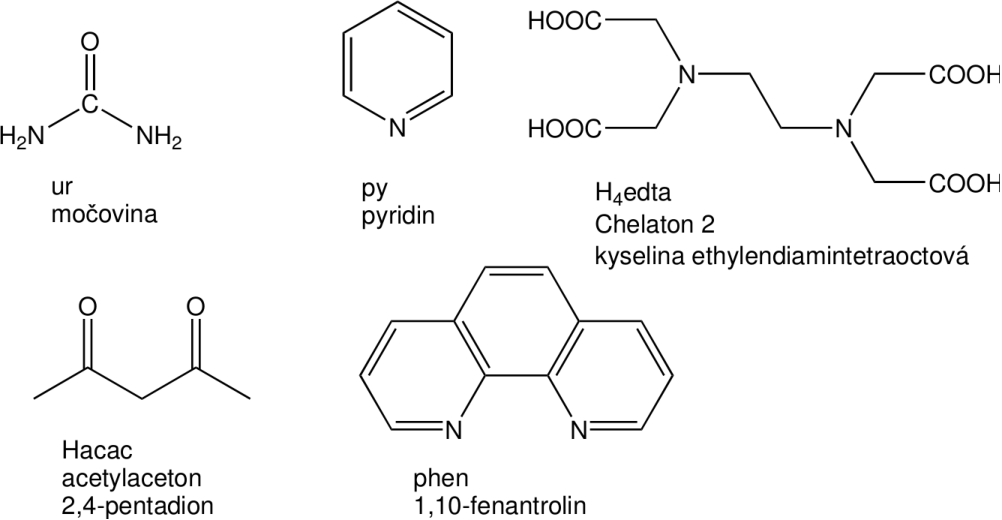
\includegraphics[keepaspectratio,width=105mm]{img/ligandy.pdf}
}

\subsubsection{Izomerie}
\frame{
	\frametitle{}
	\textbf{Izomerie}\\
	a) Ligand se koordinuje k centrálnímu atomu různými donorovými atomy. Jev se nazývá \textbf{vazebná izomerie} a izomery rozlišujeme rozdílnými názvy ligandů
	\vspace{5mm}
	\\
	\begin{tabular}{llll}
		\ce{-NO2} & nitro & \ce{-ONO} & nitrito \\
		\ce{-SCN} & thiokyanato & \ce{-NCS} & isothiokyanato \\
		\ce{-SeCN} & selenokyanato & \ce{-NCSe} & isoselenokyanato \\
	\end{tabular}
	\\
	\vspace{10mm}
	b) Koordinují se izomerní ligandy za vzniku \textbf{polohových izomerů}. I tento případ se vystihne rozdílným názvem ligandů
	\vspace{5mm}
	\\
	\begin{tabular}{ll}
		\textcolor{red}{H$_2$N}CH$_2$CH(\textcolor{red}{NH$_2$})CH$_3$ & 1,2-diaminopropan \\
		CH$_3$\textcolor{red}{NH}CH$_2$CH$_2$\textcolor{red}{NH$_2$} & N-methylethylendiamin \\
	\end{tabular}
}

\frame{
	\frametitle{}
	c) Komplex má zaměněny ionty v koordinační a iontové sféře. Tuto situaci, nazývanou \textbf{ionizační izomerie}, řeší název komplexu
	\\
	\vspace{1cm}
	\begin{tabular}{ll}
		\ce{[Co(NH3)5SO4]Br} & bromid pentaammin-sulfatokobaltitý \\
		\ce{[Co(NH3)5Br]SO4} & síran pentaammin-bromokobaltitý  \\
	\end{tabular}
	\vspace{1cm}
	\\
	d) U koordinačních sloučenin s komplexním kationtem i aniontem se může měnit rozdělení ligandů mezi koordinačními sférami obou centrálních atomů (\textbf{koordinační izomerie}) \\
	\vspace{1cm}
	\begin{tabular}{ll}
		\ce{[Pt(NH3)4][CuCl4]} & tetrachloroměďnatan tetramminplatnatý \\
		\ce{[Cu(NH3)4][PtCl4]} & tetrachloroplatnatan tetraamminměďnatý \\
	\end{tabular}
}

\frame{
	\frametitle{}
	\begin{figure}
		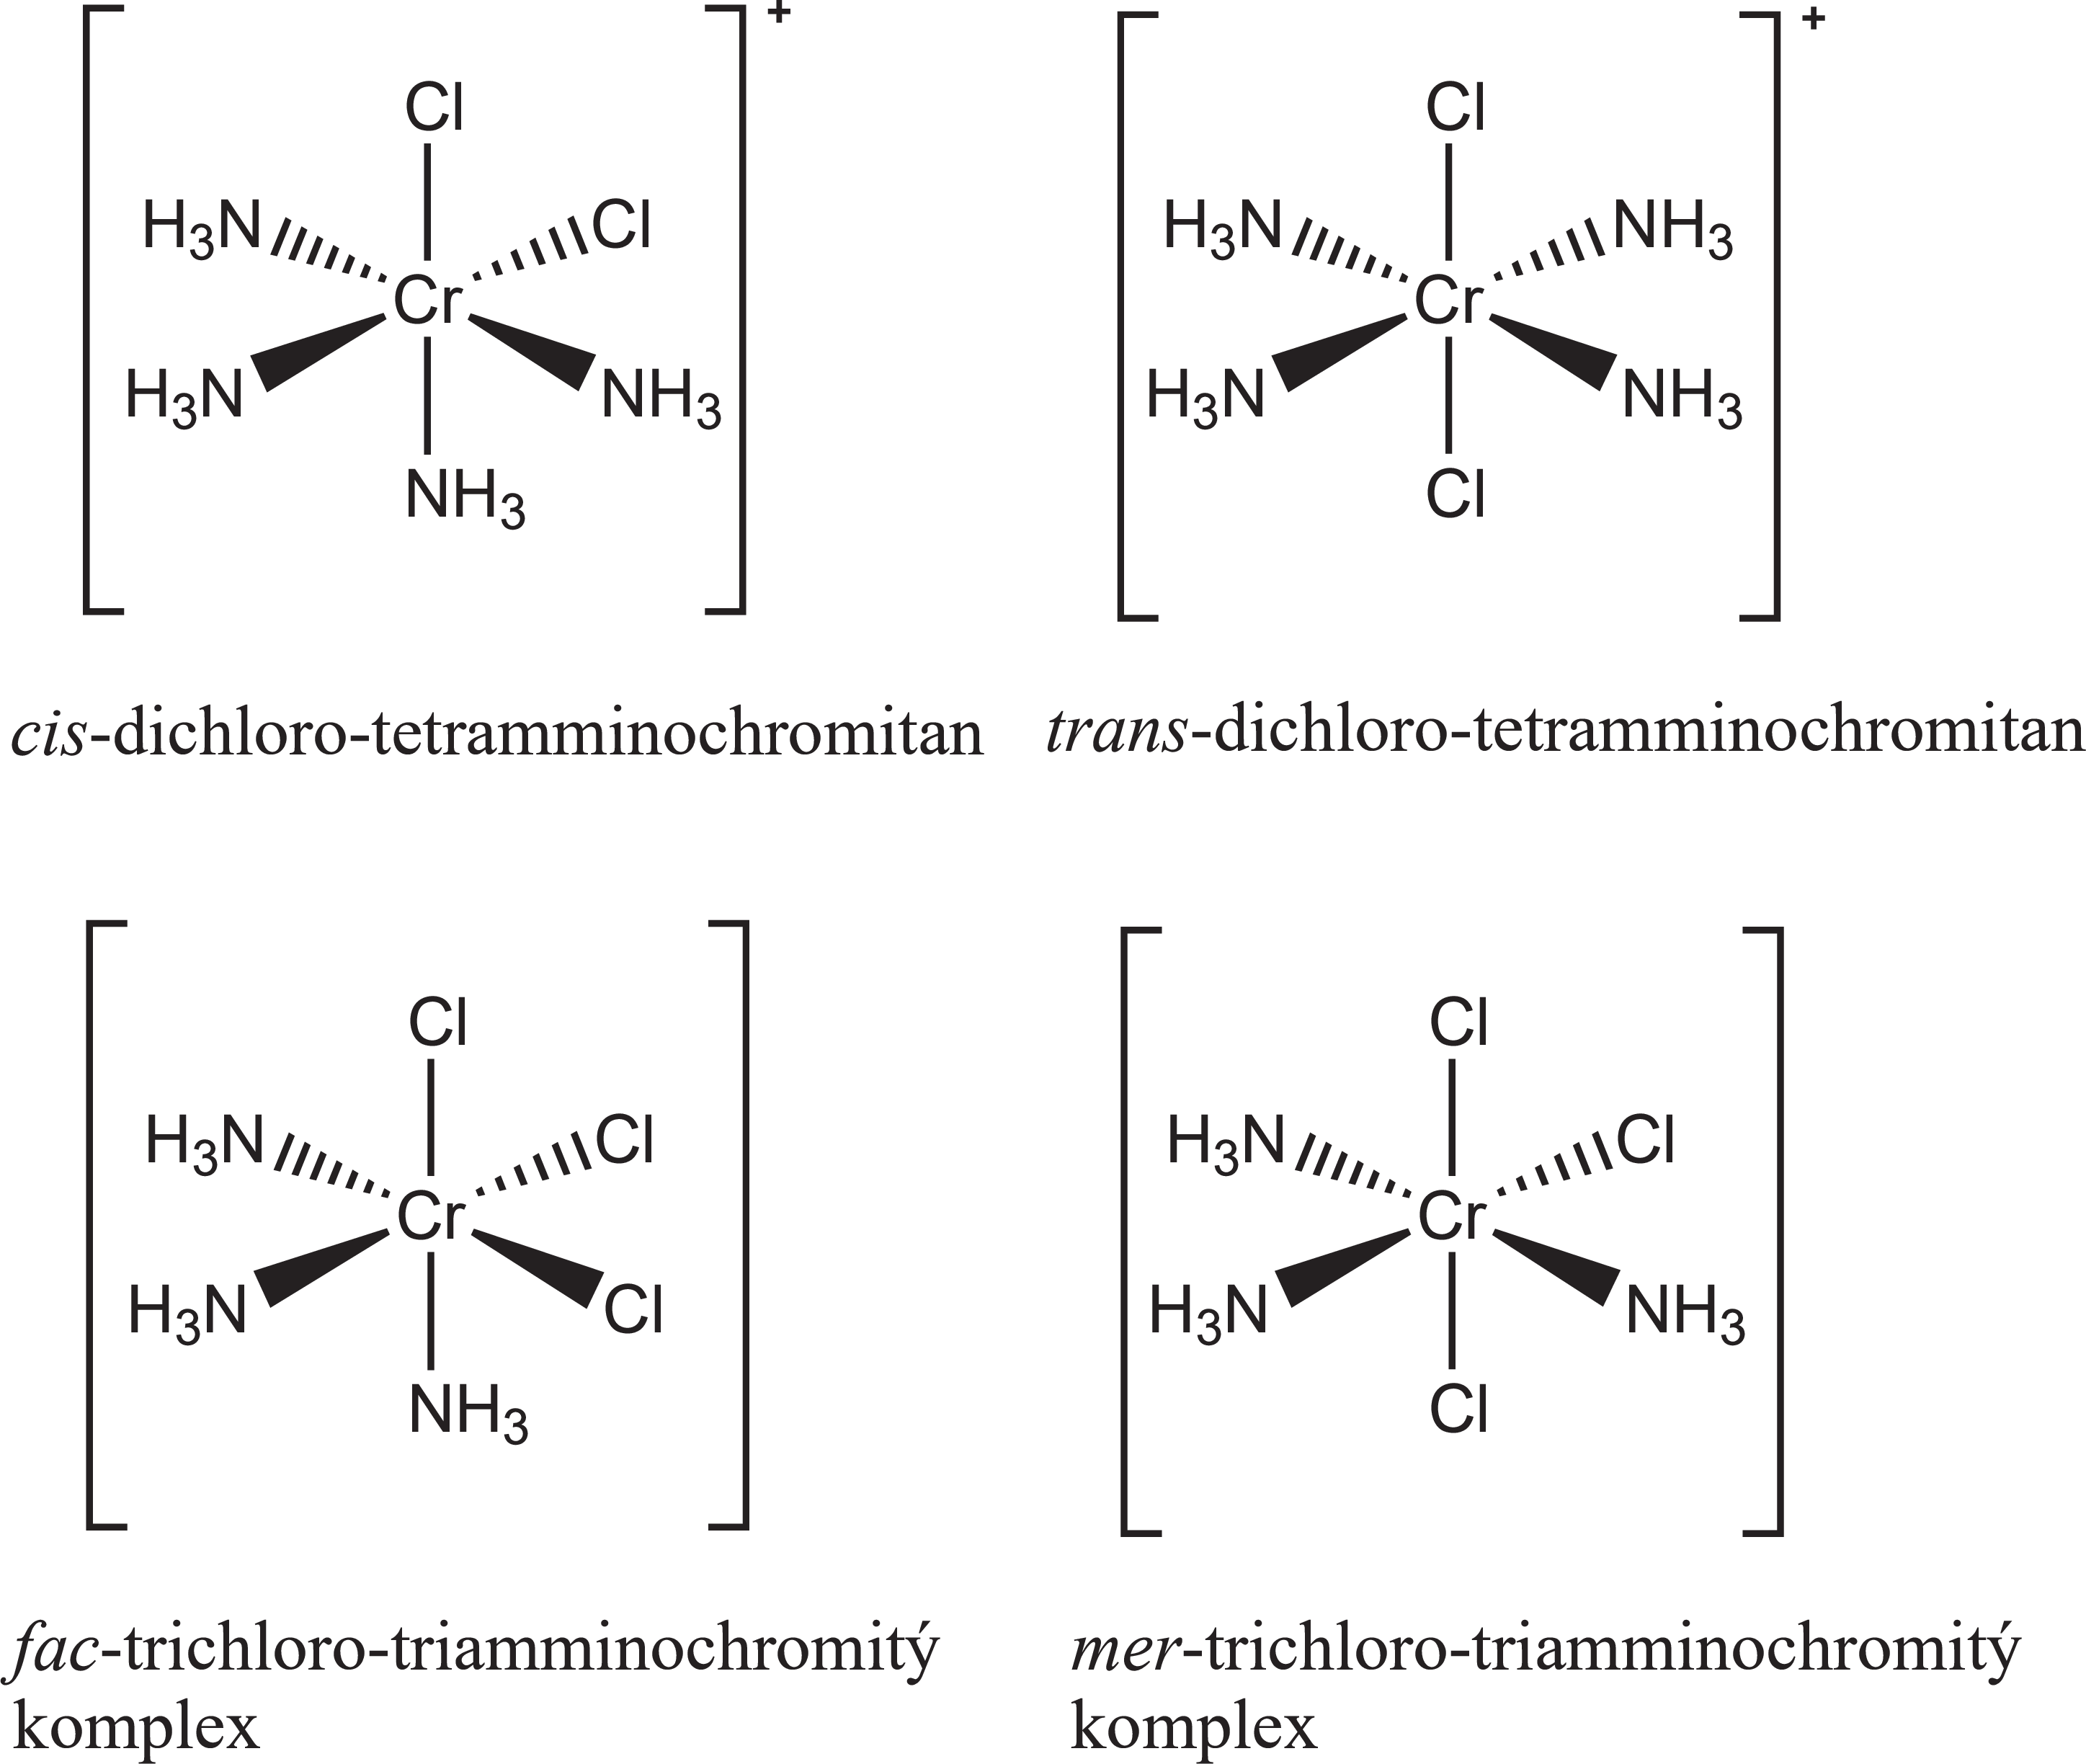
\includegraphics[height=.8\textheight]{img/izomery.png}
	\end{figure}
}

\frame{
	\frametitle{}
	\begin{itemize}
		\item Při vzniku \emph{kationtů} se uvolňují elektrony z energeticky nejvyššího obsazeného orbitalu.
		\item Při vzniku \emph{aniontů} elektrony vstupují do energeticky nejnižšího volného orbitalu.
	\end{itemize}

	\begin{tabular}{|l|l|l|l|}
		\hline
		Na & [Ne] 3s$^1$ & Na$^+$ & [Ne] (3s$^0$) \\ \hline
		Ba & [Xe] 6s$^2$ & Ba$^{2+}$ & [Xe]  (6s$^0$) \\ \hline
		Fe & [Ar] 3d$^6$ 4s$^2$ & Fe$^{3+}$ & [Ar] 3d$^5$ \\ \hline
		Cu & [Ar] 3d$^{10}$ 4s$^1$ & Cu$^{2+}$ & [Ar] 3d$^9$ \\ \hline
		S & [Ne] 3s$^2$ 3p$^4$ & S$^{2-}$ & [Ne] 3s$^2$ 3p$^6 \equiv$ [Ar] \\ \hline
		Cl & [Ne] 3s$^2$ 3p$^5$ & Cl$^-$ & [Ne] 3s$^2$ 3p$^6 \equiv$ [Ar] \\ \hline
	\end{tabular}
}

\subsection{Ligandy}
\subsubsection{Hapticita, denticita}
\frame{
	\frametitle{}
	\begin{itemize}
		\item Ligandy jsou ionty nebo molekuly, které se váží na centrální atom. Nejčastěji vystupují jako \textit{Lewisovy báze}.
		\item \emph{Denticita} - počet donorových atomů, kterými je ligand vázán k centrálnímu atomu.
		\begin{itemize}
			\item  \emph{Monodentátní ligandy} jsou vázány jedním atomem k centrálnímu kovu, např. \ce{NH3}
			\item  \emph{Bidentátní ligandy} jsou vázány dvěma atomy k centrálnímu kovu, např. ethylendiamin (en) nebo acetylaceton (acac).
		\end{itemize}
	\end{itemize}
	\begin{figure}
		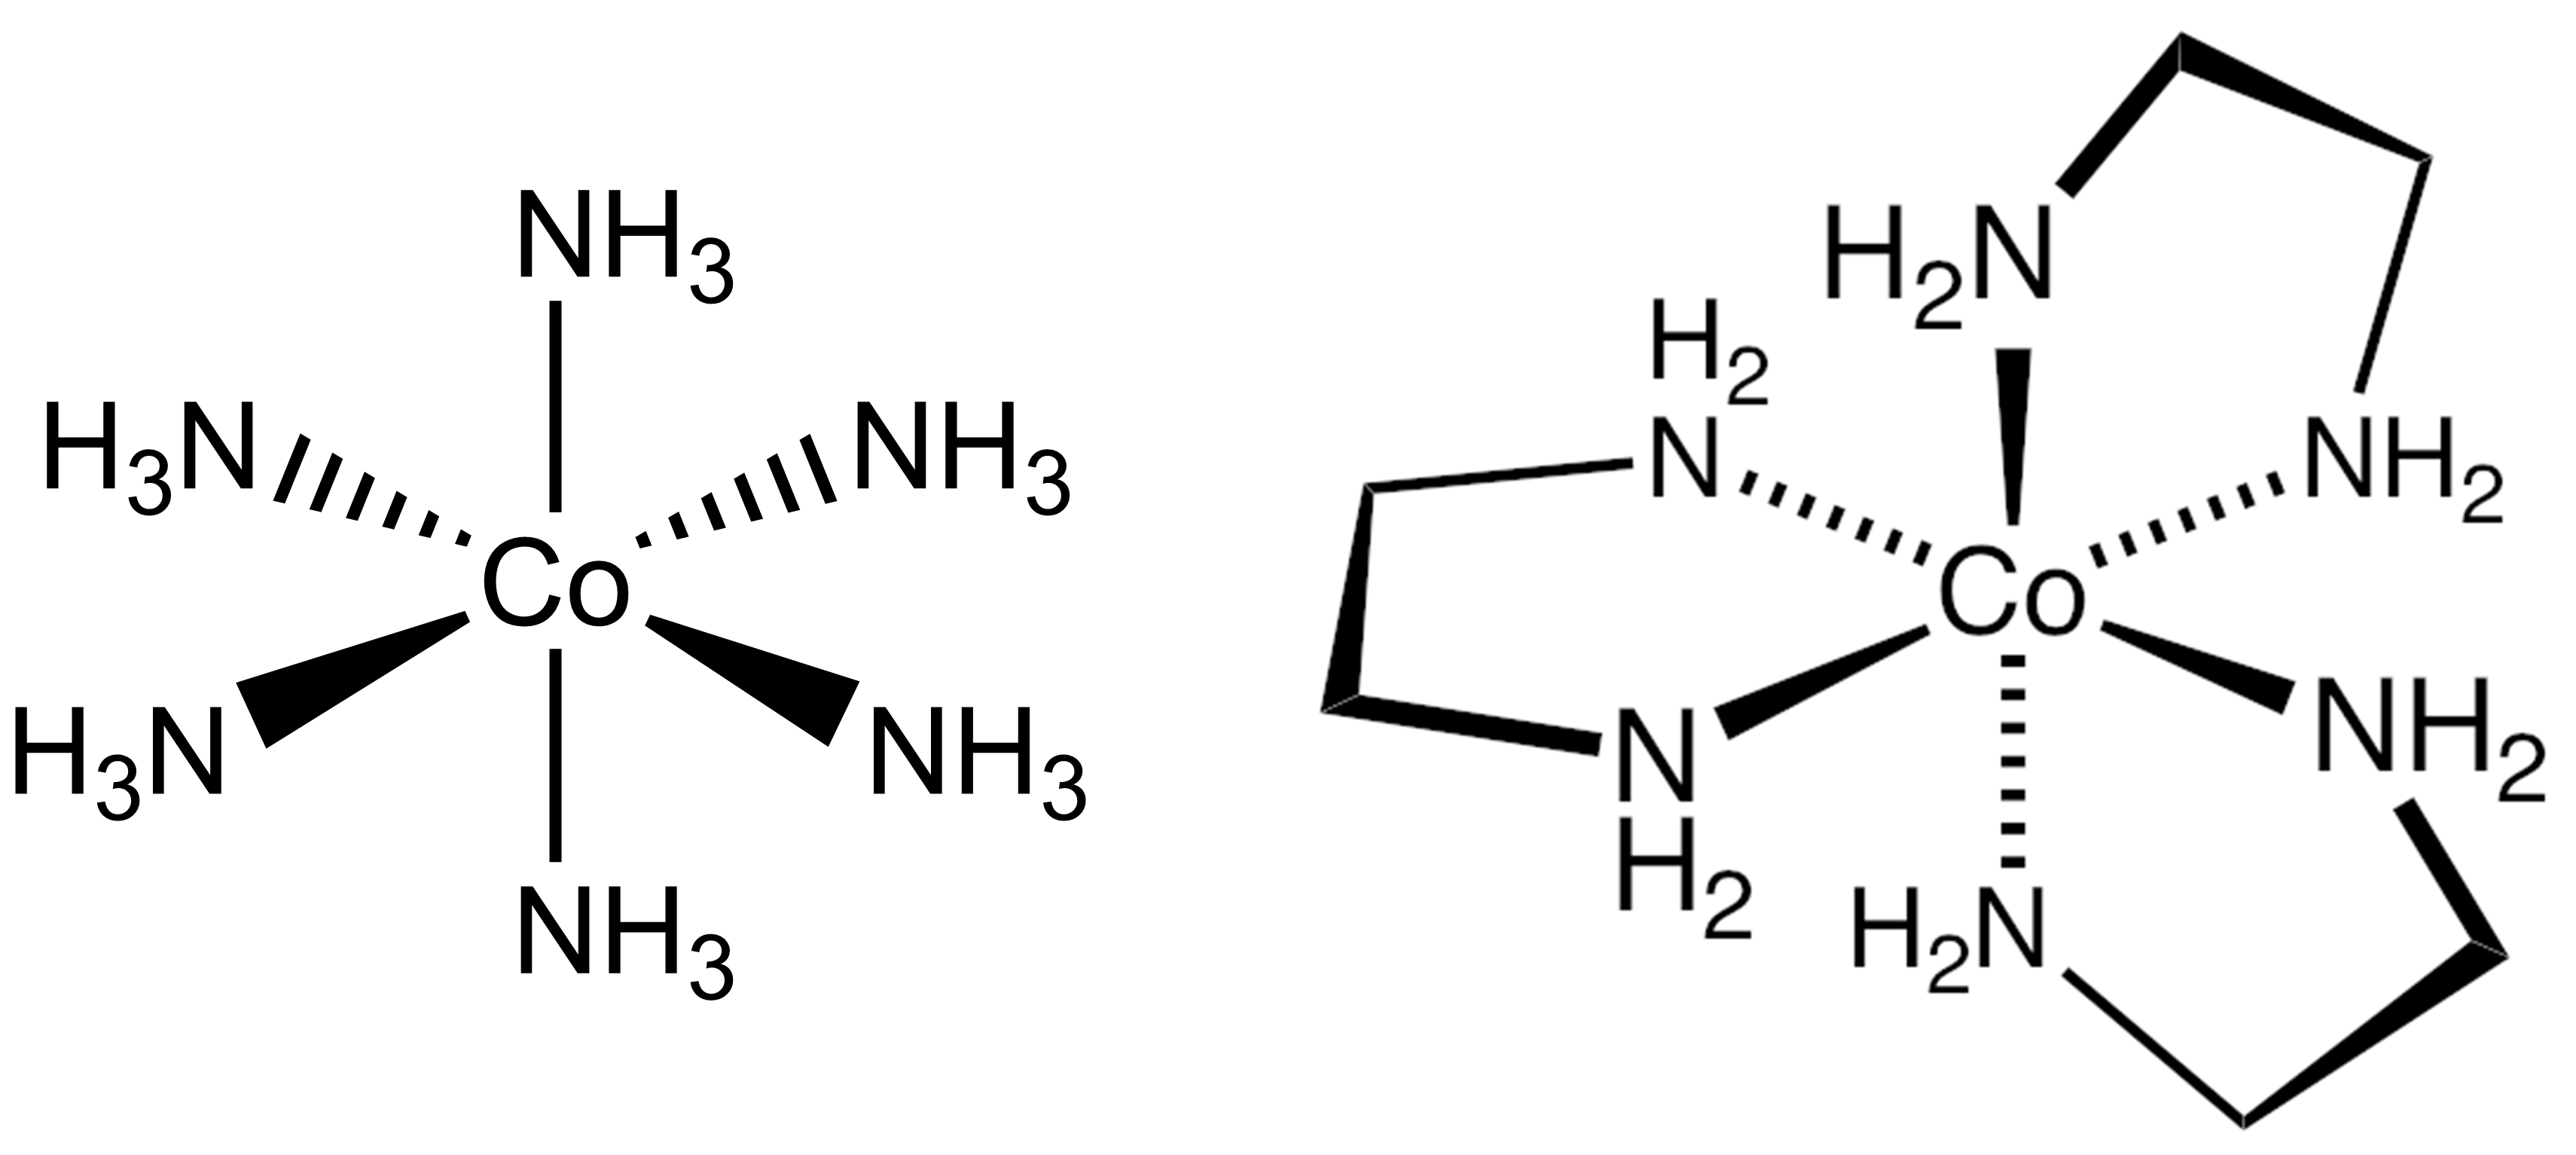
\includegraphics[width=.8\textwidth]{img/Co-denticita.png}
	\end{figure}
}

\frame{
	\frametitle{}
	\begin{itemize}
		\item \emph{Můstkový ligand} - propojuje dva nebo více centrálních atomů.
		\item Ve vzorci a názvu je před můstkovým ligandem vloženo písmeno $\mu$ s indexem vyjadřujícím počet propojených centrálních atomů.
		\item tri-$\mu_2$-karbonyl-bis(trikarbonylželezo)
	\end{itemize}
	\begin{figure}
		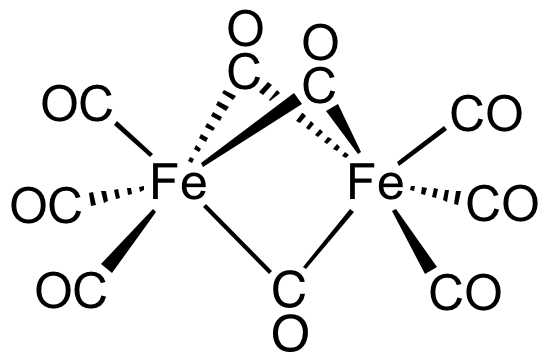
\includegraphics[height=.4\textheight]{img/Fe2-CO9.png}
	\end{figure}
}

\frame{
	\frametitle{}
	\begin{columns}
		\begin{column}{.33\textwidth}
			\begin{figure}
				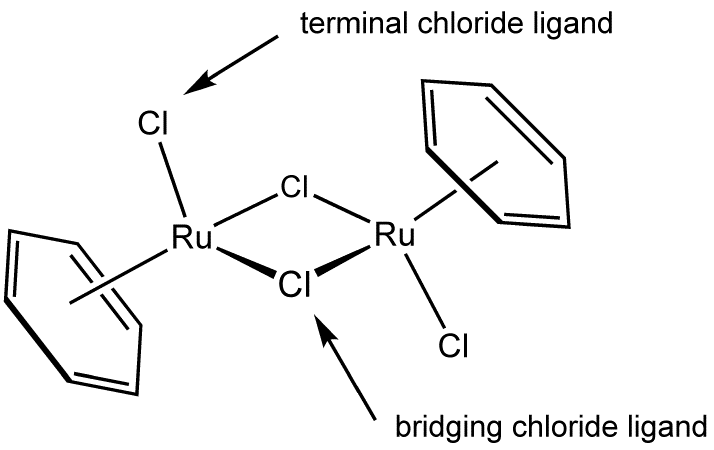
\includegraphics[width=\textwidth]{img/Ru-Cl.png}
				\caption*{$\mu_2$-Cl}
			\end{figure}
		\end{column}
		\begin{column}{.33\textwidth}
			\begin{figure}
				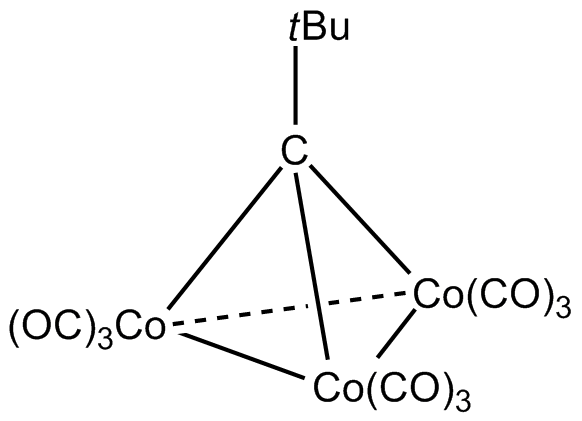
\includegraphics[width=\textwidth]{img/Mu3_compound.png}
				\caption*{$\mu_3$-C}
			\end{figure}
		\end{column}
		\begin{column}{.33\textwidth}
			\begin{figure}
				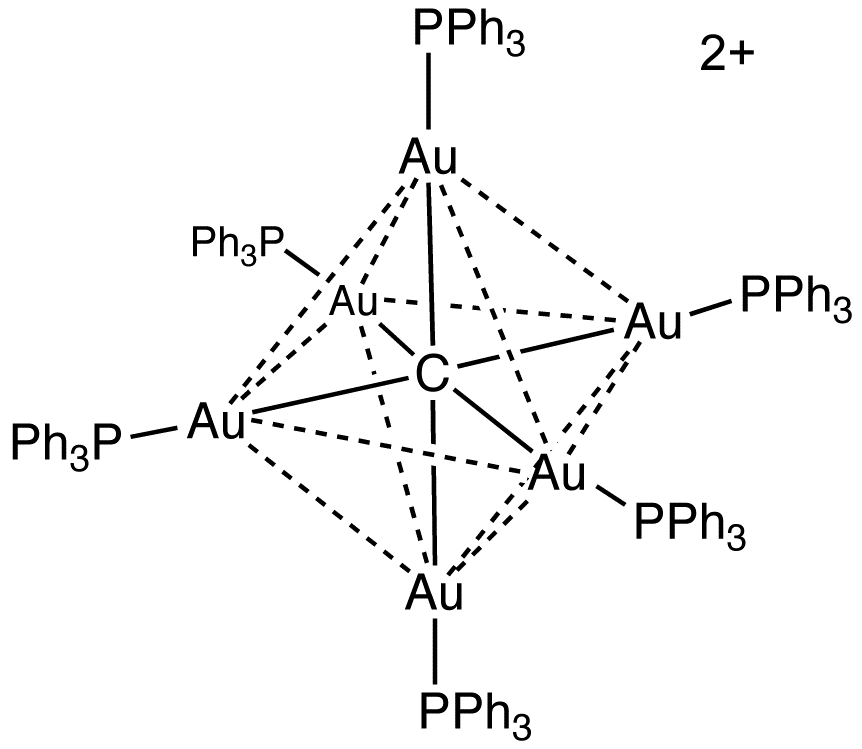
\includegraphics[width=\textwidth]{img/Au6C-PPh3-6.png}
				\caption*{$\mu_6$-C}
			\end{figure}
		\end{column}
	\end{columns}
}

\frame{
	\frametitle{}
	\begin{itemize}
		\item \emph{Hapticita} - vyjadřuje velikost (počet atomů) $\pi$-systému ligandu, kterým je vázán k centrálnímu atomu. Značí se řeckým písmenem eta ($\eta$).
		\item Ve ferrocenu je železnatý ion komplexován dvěma cyklopentadienylovými kruhy, vazba je vytvářena mezi železnatým iontem a celým $\pi$-systémem aniontu. Ligand pak označujeme jako $\eta^5$-cyklopentadienyl.
	\end{itemize}
	\begin{center}
		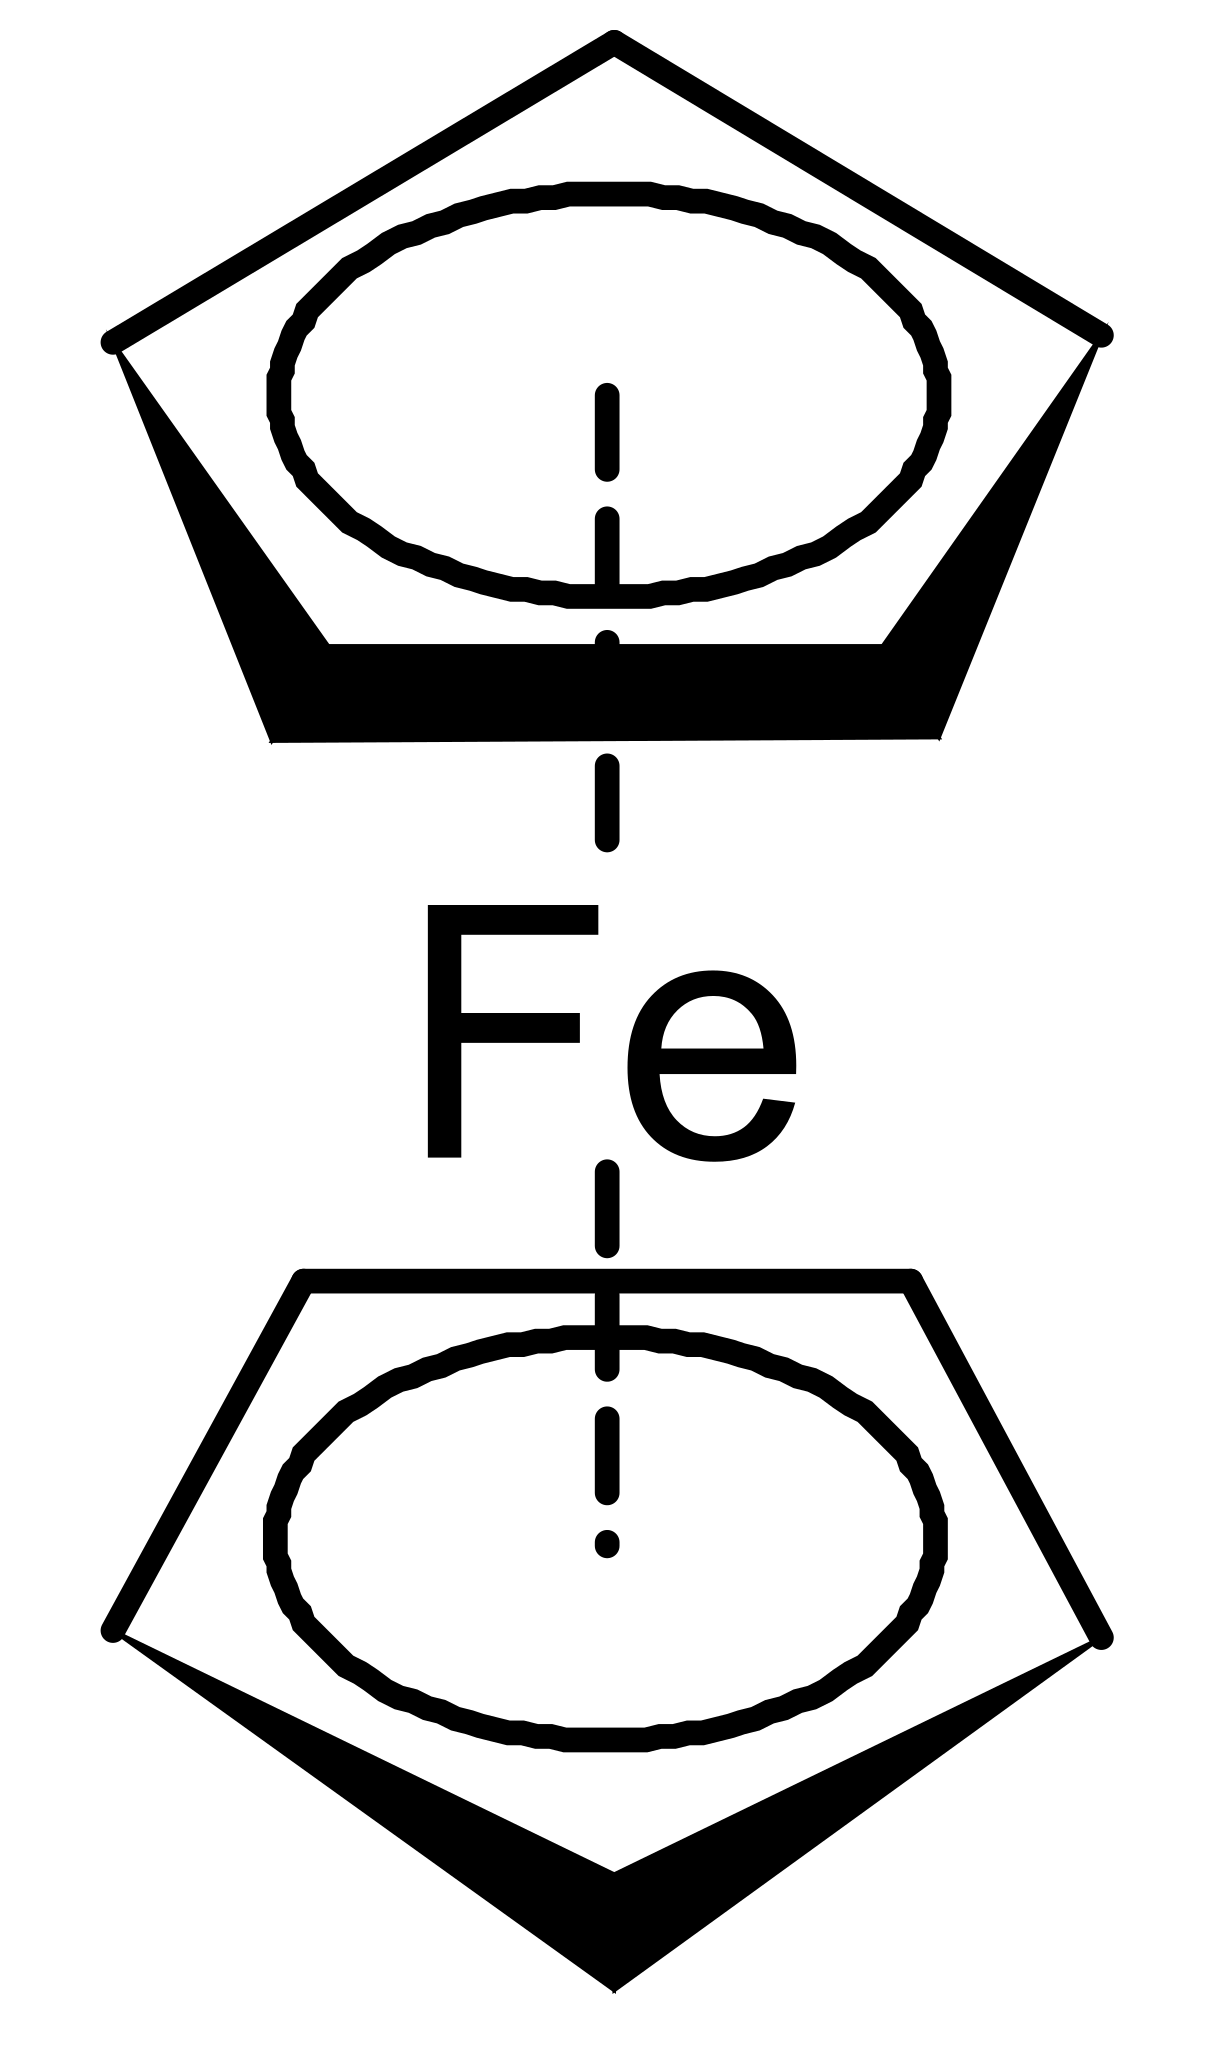
\includegraphics[height=.4\textheight]{img/ferrocen.png}
	\end{center}
}

\subsection{Konstanta stability}
\frame{
	\frametitle{}
	\vfill
	\begin{align*}
		\ce{Cu^{2+} + 4 NH3 &<=> [Cu(NH3)4]^{2+}} \\
		\ce{M + 4 L &<=> ML_4}\\
	\end{align*}
	\begin{flalign*}
		K_1 &= \frac{[ML_4]}{[ML_3] [L]} &K_2 &= \frac{[ML_3]}{[ML_2] [L]} &\\
		K_3 &= \frac{[ML_2]}{[ML] [L]} &K_4 &= \frac{[ML]}{[M] [L]} &\\
	\end{flalign*}
	\begin{flalign*}
		K &= K_1 . K_2 . K_3 . K_4 = \displaystyle\prod_{i=1}^{n} K_i = \frac{[ML_4]}{[M] [L]^4} &\\
		\Delta G^0 &= \Delta H - T\Delta S = -RT \ln K\\
	\end{flalign*}
	\vfill
}

\subsection{Chelátový efekt}
\frame{
	\frametitle{}
	\begin{columns}
		\begin{column}{.6\textwidth}
			\vfill
			\begin{itemize}
				\item Komplexy s vícedentátními ligandy jsou řádově stabilnější než komplexy s monodentátními ligandy.\footnote[frame]{\href{http://doi.wiley.com/10.1002/hlca.19520350721}{Der Chelateffekt}}
				\item Tyto komplexy se označují jako \textit{chelátové}, z řeckého chelos -- klepeto.
				\item Konstanta stability komplexu s vícevaznými ligandy je vyšší než u komplexu s jednovaznými ligandy.
				\item Nejvýraznější je tento efekt, pokud vznikají pěti- a šestičlenné cykly.\footnote[frame]{\href{https://is.muni.cz/do/rect/el/estud/pedf/js18/obecna_chemie/web/pages/15-koordinacni-slouceniny.html}{Koordinační sloučeniny}}
				\item Při vzniku chelátového komplexu nahrazením monodentátních ligandů vícedentátními dochází k výraznému zvýšení entropie systému ($+\Delta S$).
			\end{itemize}
			\vfill
		\end{column}
		\begin{column}{.4\textwidth}
			\adjincludegraphics[height=0.75\textheight]{img/Metal-EDTA.png}
		\end{column}
	\end{columns}
}

\subsection{Teorie krystalového pole (CFT)}
\frame{
	\frametitle{}
	\begin{itemize}
		\item Popisuje vazebné poměry v koordinačních sloučeninách.
		\item Interakce mezi ligandem  a centrálním kovem je popisována pomocí elektrostatiky, ligandy jsou chápány jako negativní bodové náboje a kov jako kladný náboj.
		\item Vazba je realizována pomocí d-orbitalů kovu, které jsou v nevázaném iontu energeticky \emph{degenerované}, tzn. mají stejnou energii.
		\item Po vytvoření komplexu dojde, v závislosti na tvaru komplexu, k jejich rozštěpení na dvě skupiny. Velikost rozštěpení (rozdíl energií) je dána několika faktory:
		\begin{itemize}
			\item povahou a oxidačním stavem kovového iontu, čím je vyšší oxidační stav kovu, tím pozorujeme i silnější štěpení
			\item geometrickým uspořádáním ligandů okolo centrálního kovu
			\item povahou ligandu, čím silněji ovlivňuje ligand centrální kov, tím bude štěpení silnější
		\end{itemize}
		\item Sílu štěpení můžeme odhadnout pomocí spektrochemické řady ligandů, což je výčet ligandů seřazený podle síly generovaného pole:
		\begin{itemize}
			\item \ce{S^{2-}} $<$ \ce{SCN^{–}} $<$ \ce{Cl^{–}} $<$ \ce{F^{–}} $<$ \ce{OH^{–}} $<$ \ce{H2O} $<$ \ce{NH3} $<$ \ce{CN^{–}} $<$ \ce{CO}
		\end{itemize}
	\end{itemize}
}


\subsubsection{d-orbitaly}
\frame{
	\frametitle{}
	\begin{itemize}
		\item Existuje pět atomových d-orbitalů, podle symetrie je můžeme rozdělit na dvě skupiny:
		\begin{itemize}
			\item \emph{t$_{2g}$} – sem patří tři orbitaly, jejichž laloky leží mezi osami souřadného systému, tj. $d_{xy}$, $d_{yz}$ a $d_{xz}$
			\item \emph{e$_g$} – dva orbitaly, jejichž laloky leží v osách souřadného systému, tj. $d_{z^2}$ a $d_{x^2-y^2}$.
		\end{itemize}
	\end{itemize}
	\begin{figure}
		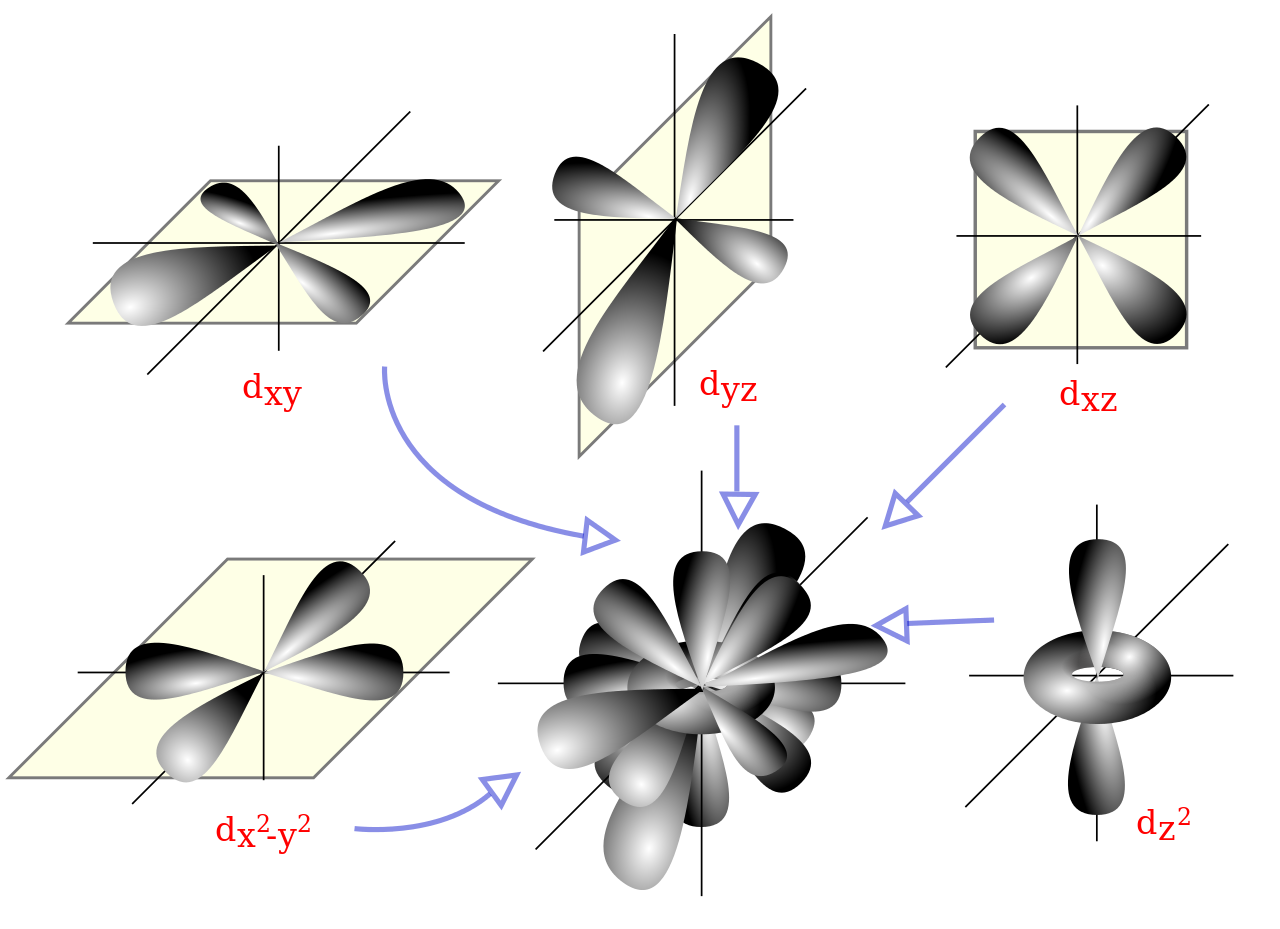
\includegraphics[height=.4\textheight]{img/d-orbitals.png}
		\caption*{Tvary d-orbitalů.\footnote[frame]{\href{https://commons.wikimedia.org/wiki/File:D_orbitals.svg}{Zdroj: Sven/Commons}}}
	\end{figure}
}

\subsection{Teorie ligandového pole}
\frame{
	\frametitle{}
	\begin{itemize}
		\item Kombinace CFT a teorie molekulových orbitalů.\footnote[frame]{\href{http://pubs.rsc.org/en/content/articlelanding/1957/qr/qr9571100381}{Ligand Field Theory}}
		\item Byla formulována roku 1957 Griffithem a Orgelem.[2]
		\item Teorie využívá elektrostatické interakce pro popis chování kovových iontů v roztoku a molekulových orbitalů pro popis rozdílů v interakcích mezi ligandy a kovem.
		\item Umožňuje odvodit barevnost a magnetické vlastnosti komplexů.
		\begin{itemize}
			\item \textit{Barevnost} je způsobena absorpcí části viditelného spektra. Během ní dochází k excitaci elektronu z t$_{2g}$ orbitalu do e$_{g}$.
			\item \textit{Magnetické vlastnosti} závisí na přítomnosti (\textit{paramagnetické komplexy}) nebo nepřítomnosti (\textit{diamagnetické komplexy}) nespárovaných elektronů.
		\end{itemize}
	\end{itemize}
}

\subsubsection{Multiplicita}
\frame{
	\frametitle{}
	\textbf{Multiplicita}
	\begin{itemize}
		\item Popisuje počet nepárových elektronů v komplexu.
		\item Je dána vztahem: M = 2S + 1, kde S je celkový spin komplexu.
	\end{itemize}

	\begin{tabular}{|l|l|l|l|}
		\hline
		\textbf{Počet nespárovaných elektronů} & \textbf{S} & \textbf{M} & \textbf{Označení} \\\hline
		0 & 0 & 1 & singlet \\\hline
		1 & $\frac{1}{2}$ & 2 & dublet \\\hline
		2 & 1 & 3 & triplet \\\hline
		3 & $\frac{3}{2}$ & 4 & kvartet \\\hline
		4 & 2 & 5 & kvintet \\\hline
		5 & $\frac{5}{2}$ & 6 & sextet \\\hline
		6 & 3 & 7 & septet \\\hline
	\end{tabular}
}

\subsubsection{Štěpení v oktaedrickém poli}
\frame{
	\frametitle{}
	\textbf{Štěpení v oktaedrickém poli}
	\begin{itemize}
		\item Komplex se skládá z centrálního atomu a šesti ligandů, které jsou umístěny ve vrcholech oktaedru.
		\item Orbitaly $e_g$ si zvýší energii oproti neštěpeným d-orbitalům a orbitaly $t_{2g}$ si ji naopak sníží.\footnote[frame]{\href{https://chem.libretexts.org/Courses/University_of_California_Davis/UCD_Chem_002C/UCD_Chem_2C\%3A_Larsen/Text/Unit_2\%3A_Coordination_Chemistry/2.08\%3A_Bonding_in_Complex_Ions\%3A_Crystal_Field_Theory}{Bonding in Octahedral Complex Ions: Crystal Field Theory}}
		\item Rozdíl mezi energetickými hladinami označujeme jako stabilizační energii oktaedrického pole ($\Delta_O$).
		\item V případě silných ligandů je hodnota $\Delta_O$ vyšší než hodnota párovací energie v d-orbitalech, proto se nejprve zcela zaplní orbitaly $t_{2g}$ a až poté se začnou plnit orbitaly $e_g$, vznikají tzv. \emph{nízkospinové komplexy}.
	\end{itemize}
	\begin{center}
		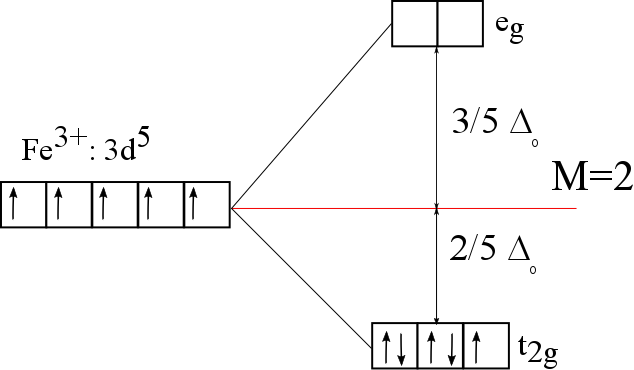
\includegraphics[keepaspectratio,width=40mm]{img/oktaedr-nizkospinovy.png}
	\end{center}
}

\frame{
	\frametitle{}
	\begin{center}
		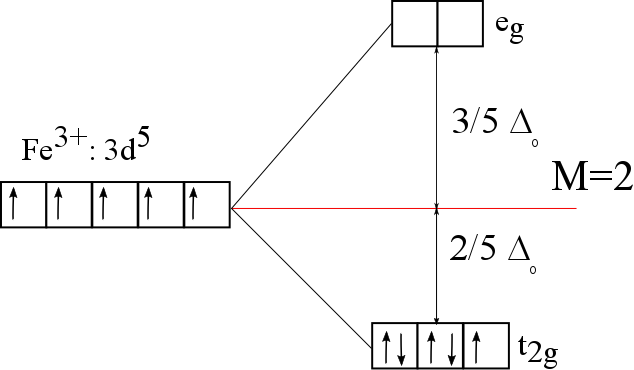
\includegraphics[keepaspectratio,width=110mm]{img/oktaedr-nizkospinovy.png}
	\end{center}
}

\frame{
	\frametitle{}
	\begin{itemize}
		\item V případě slabých ligandů je hodnota $\Delta_O$ nižší než hodnota párovací energie v d-orbitalech, pak je pro elektrony výhodnější nejprve zpola zaplnit všech pět orbitalů a až poté doplňovat elektronové páry v orbitalech. Vznikají tzv. \emph{vysokospinové komplexy}.
	\end{itemize}
	\begin{center}
		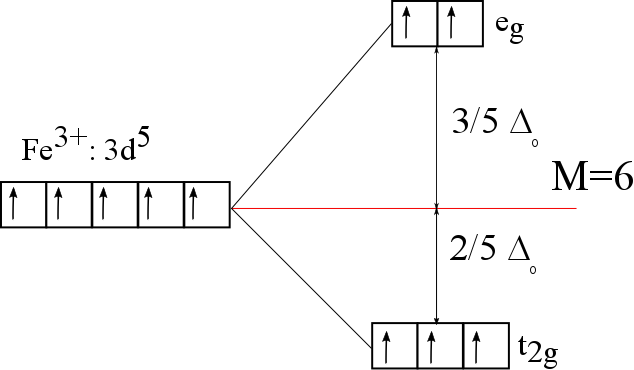
\includegraphics[keepaspectratio,width=80mm]{img/oktaedr-vysokospinovy.png}
	\end{center}
}

\subsubsection{Štěpení v tetraedrickém poli}
\frame{
	\frametitle{}
	\textbf{Štěpení v tetraedrickém poli}
	\begin{itemize}
		\item Komplex se skládá z centrálního atomu a čtyř ligandů, které jsou umístěny ve vrcholech tetraedru.
		\item Štěpení orbitalů je opačné, $e_g$ jdou energeticky dolů a $t_{2g}$ nahoru.
		\item Síla tetraedrického pole ($\Delta_t$) je menší než polovina oktaedrického pole (přesně jde o $\frac{4}{9}\Delta_O$), proto jsou všechny tetraedrické komplexy \textit{vysokospinové}.
	\end{itemize}
	\begin{center}
		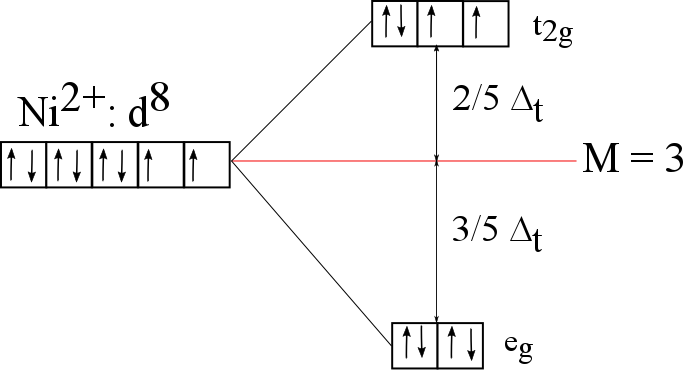
\includegraphics[keepaspectratio,width=80mm]{img/tetraedr-vysokospinovy.png}
	\end{center}
}

\subsection{Jahnův-Tellerův efekt}
\frame{
	\frametitle{}
	\begin{exampleblock}{}
		{\large ``Každá nelineární molekula, která má elektrony v degenerovaném stavu, bude nestálá a bude se deformovat tak, aby vznikl systém o nižší energii, v němž bude degenerace odstraněna.''}
		\vskip5mm
		\hspace*\fill{\small--- Jahnův-Tellerův teorém}
	\end{exampleblock}
	\begin{itemize}
		\item S tímto jevem se můžeme setkat např. u oktaedrických komplexů iontů d$^4$ a d$^9$, např. u \ce{CuF2}, který je tvořen oktaedrickými jednotkami \ce{CuF6}.\footnote[frame]{\href{https://doi.org/10.1021/ja01562a011}{The Crystal Structure of Copper(II) Fluoride}}
		\item V tomto oktaedrickém komplexu jsou d-orbitaly rozštěpeny na dvě sady, t$_{2g}$ a e$_g$, vlivem tohoto efektu dojde k dalšímu štěpení d-orbitalů a tím, k jejich energetické stabilizaci.
		\item U oktaedrických komplexů může dojít buď k jejich protažení zkrácení.
	\end{itemize}
}

\frame{
	\frametitle{}
	\begin{itemize}
		\item V případě protažení axiálních vazeb (ležících v ose z), dojde ke snížení energie d-orbitalů s komponentou z (d$_{xz}$, d$_{yz}$ a d$_z^2$), zbylé orbitaly si energii zvýší. V případě zkrácení to bude naopak.
	\end{itemize}
	\begin{center}
		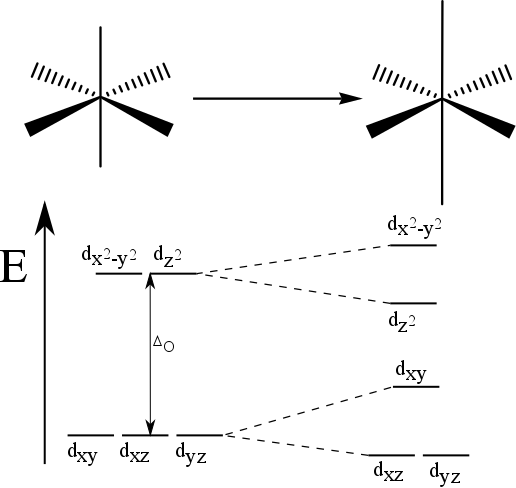
\includegraphics[keepaspectratio,height=0.6\textheight]{img/jahn-teller.png}
	\end{center}
}

\section{Supertěžké prvky}
\frame{
	\frametitle{}
	Supertěžké prvky mají protonové číslo vyšší než 103.
	\begin{tabular}{|l|l|l|r@{ }l|}
		\hline
		\textbf{Z} & \textbf{Značka} & \textbf{Název} & \multicolumn{2}{|c|}{\textbf{$T_{\frac{1}{2}}$}} \\\hline
		104 & Rf & Rutherfordium & 1,3 &h \\\hline
		105 & Db & Dubnium & 28 &h \\\hline
		106 & Sg & Seaborgium & 14 &min \\\hline
		107 & Bh & Bohrium & 11,5 &min \\\hline
		108 & Hs & Hassium & 110 &s \\\hline
		109 & Mt & Meitnerium & 67 &s \\\hline
		110 & Ds & Darmstadtium & 14 &s \\\hline
		111 & Rg & Roentgenium & 306 &s \\\hline
		112 & Cn & Copernicium & 28 &s\\\hline
		113 & Nh & Nihonium & 9,5 &s \\\hline
		114 & Fl & Flerovium & 19 &s \\\hline
		115 & Mc & Moscovium & 650 &ms \\\hline
		116 & Lv & Livermorium & 57 &ms \\\hline
		117 & Ts & Tennessine & 51 &ms \\\hline
		118 & Og & Oganesson &  181 &ms \\\hline
	\end{tabular}
}

\frame{
	\frametitle{}
	\begin{figure}
		\adjincludegraphics[width=1.1\textwidth]{../IUPAC_PSP.jpg}
	\end{figure}
}

\subsection{Dokončení 7. periody}
\frame{
	\frametitle{}
	\vfill
	\begin{itemize}
		\item Organizace IUPAC vydala 9.6. 2016 návrh na pojmenování nových čtyř prvků s protonovými čísly 113, 115, 117 a 118.\footnote[frame]{\href{https://iupac.org/iupac-is-naming-the-four-new-elements-nihonium-moscovium-tennessine-and-oganesson/}{IUPAC is naming the four new elements nihonium, moscovium, tennessine, and oganesson}}
		\item 28. 11. 2016 byly tyto názvy schváleny.\footnote[frame]{\href{https://iupac.org/iupac-announces-the-names-of-the-elements-113-115-117-and-118/}{IUPAC announces the names of the elements 113, 115, 117, and 118}}$^,$\footnote[frame]{\href{https://www.osel.cz/8881-dalsi-ctyri-supertezke-prvky-maji-sva-jmena.html}{Další čtyři supertěžké prvky mají svá jména}}
		\item Všechny tyto nově připravené prvky jsou nestabilní, jejich poločasy rozpadu se pohybují ve zlomcích sekund.
		\item Kromě metod přípravy jsou studovány i jejich chemické vlastnosti.\footnote[frame]{\href{https://doi.org/10.1515/ract-2022-0015}{Five decades of GSI superheavy element discoveries and chemical investigation}}
	\end{itemize}
	\begin{tabular}{|c|c|c|}
		\hline
		\textbf{Protonové číslo} & \textbf{Původní název} & \textbf{Schválený název} \\
		\hline
		113 & Ununtrium (Uut) & Nihonium (Nh) \\
		\hline
		115 & Ununpentium (Uup) & Moscovium (Mc) \\
		\hline
		117 & Ununseptium (Uus) & Tennessine (Ts) \\
		\hline
		118 & Ununoctium (Uuo) & Oganesson (Og) \\
		\hline
	\end{tabular}
	\vfill
}

\subsection{Hledání dalších supertěžkých prvků}
\frame{
	\frametitle{}
	\begin{columns}
		\begin{column}{.6\textwidth}
			\vfill
			\begin{itemize}
				\item Struktura atomového jádra je podobná struktuře elektronového obalu.
				\item Protony mají svůj systém hladin, stejně tak neutrony. Z toho důvodu existují velmi stabilní kombinace počtu protonů a neutronů, tzv. \textit{magická čísla}, kdy jsou tyto slupky zcela zaplněny.
				\item 2, 8, 20, 28, 50, 82, 126\footnote[frame]{\href{https://oeis.org/A018226}{Magic numbers of nucleons}}
				\item U těchto číselných kombinací se očekává zvýšená stabilita jader.
				\item Stabilitu jader dále zvyšuje sudý počet protonů i neutronů.
			\end{itemize}
			\vfill
		\end{column}
		\begin{column}{.4\textwidth}
			\begin{figure}
				\adjincludegraphics[height=0.6\textheight]{img/Table_isotopes_en.png}
				\caption*{Typ rozpadu jádra v závislosti na protonovém čísle.\footnote[frame]{Zdroj: \href{https://commons.wikimedia.org/wiki/File:Table_isotopes_en.svg}{Napy1kenobi/Commons}}}
			\end{figure}
		\end{column}
	\end{columns}
}

\frame{
	\frametitle{}
	\vfill
	\begin{itemize}
		\item V oblasti okolo magických čísel se očekávají tzv. \textit{ostrovy stability}.\footnote[frame]{\href{https://www.osel.cz/11733-novinky-ve-studiu-velmi-tezkych-a-supertezkych-prvku.html}{Novinky ve studiu velmi těžkých a supertěžkých prvků}}
		\item Přesnou polohu těchto ostrovů je obtížné určit, každé nově objevené jádro pomáhá zpřesnit modely.\footnote[frame]{\href{http://www.chemicke-listy.cz/ojs3/index.php/chemicke-listy/article/view/3334}{Meze periodické tabulky}}
		\item První ostrov stability se předpokládá v blízkosti jádra $^{298}_{114}$Fl.
		\item Příprava těchto jader je ovšem velmi komplikovaná, např.:
		\item \ce{^{248}_{94}Pu + ^{50}_{20}Ca -> ^{298}_{114}Fl}
		\item \ce{^{248}_{96}Cm + ^{238}_{92}U -> ^{298}_{114}Fl + ^{186}_{74}W + 2 ^1_0n}
		\item Druhý ostrov stability se předpokládá až u protonového čísla 164, to je ale se současnou technologií nedosažitelné.\footnote[frame]{\href{https://doi.org/10.1007/BF01406719}{Investigation of the stability of superheavy nuclei around Z=114 and Z=164}}
	\end{itemize}
	\vfill
}

\frame{
	\frametitle{}
	\vfill
	\begin{figure}
		\adjincludegraphics[height=0.65\textheight]{img/Island_of_Stability.png}
		\caption*{Ostrovy stability.\footnote[frame]{Zdroj: \href{https://commons.wikimedia.org/wiki/File:Island_of_Stability.svg}{InvaderXan/Commons}}}
	\end{figure}
	\vfill
}

\frame{
	\frametitle{}
	\vfill
	\begin{itemize}
		\item Nová supertěžká jádra lze produkovat několika způsoby:\footnote[frame]{\href{https://www.osel.cz/8666-jak-se-produkuji-a-studuji-supertezke-prvky.html}{Jak se produkují a studují supertěžké prvky}}
		\begin{enumerate}
			\item Ostřelováním těžkých jader intenzivním proudem neutronů, např.:
			\begin{itemize}
				\item \ce{^{238}_{92}U + ^1_0n -> ^{239}_{92}U ->[23 min] ^{239}_{93}Np + $\beta^-$ ->[56 hod] ^{239}_{94}Pu + $\beta^-$}
			\end{itemize}
			\item Ostřelováním terče s obsahem těžkých, stabilních jader jiným těžkým jádrem.
			\begin{itemize}
				\item \ce{^{64}_{28}Ni + ^{209}_{83}Bi -> ^{272}_{111}Rg + ^1_0n}
				\item \ce{^{70}_{30}Zn + ^{208}_{82}Pb -> ^{277}_{112}Cn + ^1_0n}
			\end{itemize}
		\end{enumerate}
		\item Výzkum nových prvků probíhá v několika laboratořích:
		\begin{itemize}
			\item Joint Institute for Nuclear Research v Dubně\footnote[frame]{\href{http://www.jinr.ru/main-en/}{Joint Institute for Nuclear Research}}
			\item Riken v Japonsku\footnote[frame]{\href{https://www.riken.jp/en/}{RIKEN}}
			\item GSI Helmholtz Centre for Heavy Ion Research v Darmstadtu\footnote[frame]{\href{https://www.gsi.de/start/aktuelles.htm}{GSI}}
		\end{itemize}
	\end{itemize}
	\vfill
}

\frame{
	\frametitle{}
	\vfill
	\begin{itemize}
		\item Syntéza prvních prvků 8. periody je již studována.
		\item \textbf{Ununennium}, Uue, prvek 119
		\begin{itemize}
			\item První neúspěšný pokus byl proveden již v roce 1985\footnote[frame]{\href{https://doi.org/10.1103/PhysRevC.32.1760}{Search for superheavy elements using the $^{48}$Ca+$^{254}$Es$^g$ reaction}}
			\item \ce{^{254}_{99}Es + ^{48}_{20}Ca -> ^{302}_{119}Uue^*}
			\item Nadějnější se zdá experiment z roku 2020 (Riken, Japonsko):\footnote[frame]{\href{https://www.nature.com/articles/d41586-019-00285-9}{Extreme chemistry: experiments at the edge of the periodic table}}
			\item \ce{^{248}_{96}Cm + ^{51}_{23}V -> ^{299}_{119}Uue^*}
		\end{itemize}
		\item \textbf{Unbibium}, Ubb, prvek 122
		\begin{itemize}
			\item V roce 2000 se o syntézu pokoušeli v GSI:\footnote[frame]{\href{https://doi.org/10.1103/PhysRevC.98.024308}{Investigations of the synthesis of the superheavy element Z = 122}}
			\item \ce{^{238}_{92}U + ^{65}_{29}Cu -> ^{303}_{121}Ubu^*}
		\end{itemize}
		\item Cesta k těžším prvkům zatím není zcela zřejmá.
		\item Jednou z exotičtějších možností je studium prvků vyvržených během exploze supernovy.\footnote[frame]{\href{https://www.scientificamerican.com/article/superheavy-elements-are-breaking-the-periodic-table/}{Superheavy Elements Are Breaking the Periodic Table}}
	\end{itemize}
	\vfill
}

\input{../Last}

\end{document}